%Results

\subsubsection*{Division of labour}
Our model is able to simulate the divison of labour. In Fig.\ref{fig:thetax} on the left we see the development of the thresholds $\theta_{ij}$ as a function of time. For each individuum $i$ there is one line with respect to each task $j$. Here, we have used N=5 bees and M=2 tasks, amounting to 10 depicted lines - one line for each task for each bee. We can see that in the beginning the values of $\theta_{ij}$ oscillate and then assume a steady state from approximately $t=3000$ on. In this steady state, exactly five lines assume the constant maximum value $\theta_{ij}=1000$ and five lines assume the constant minimum value $\theta_{ij}=0$. This means that the five bees specialize in exactly one task and keep performing this single task in the steady state.

\begin{figure}[ht!]
	\centering
	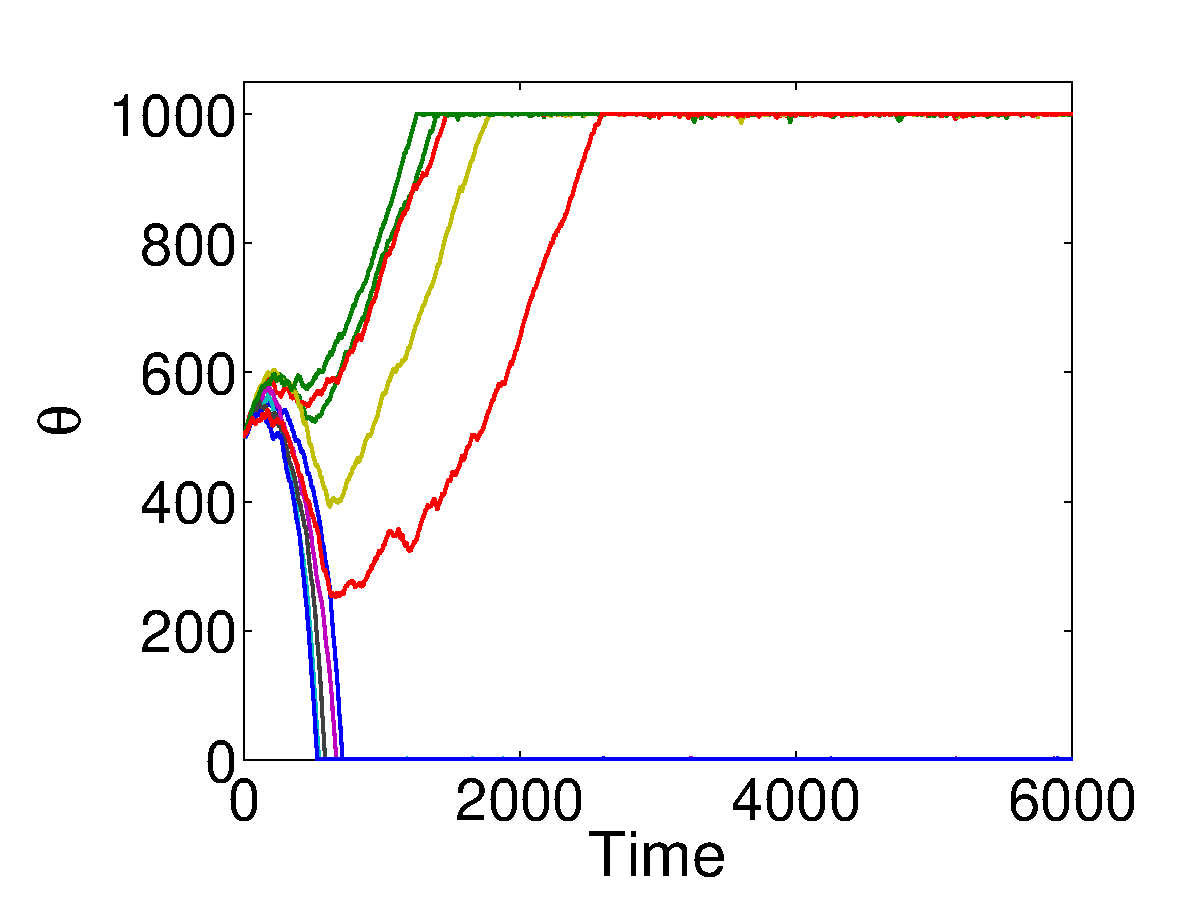
\includegraphics[width=0.4\textwidth]{../figures/thetax.eps}
	\caption{$\theta$ as a function of time.}
	\label{fig:thetax}
\end{figure}

This behaviour can be explained as follows. In the beginning, the five bees have no preference for any task as their $\theta=500$ for all tasks. In other words, there is no specialization yet. First, a bee tries out to perform one of the two tasks and gets inactive with a certain probability over time. It might subsequently decide to continue pursuing its first task or alternatively perform the second one. This decision is influenced by two factors. First, by the choice of the other bees. If all bees perform task 1, the stimulus for this task will be negligible compared to the increasing stimulus for task 2 and it becomes more likely to perform this second task. Second, by the skills the bee has gained or forgotten with respect to a specific task. The more time a bee spends pursuing task 1, the better it gets performing it. In our model, the bee is then more likely to continue pursuing this task. Vice versa is true for a task which is not performed regularly by a bee. Therefore, what we observe is that some bees will exclusively perform task 1, thus $\theta_{j=1}=0$ and $\theta_{j=2}=1000$ in the steady state, and others decide to perform task 2, thus $\theta_{j=2}=0$ and $\theta_{j=1}=1000$. The model consequently allows for the investigation of the division of labour in societies. Driving force for the division is the specialization by a learning and forgetting process.
In Fig.\ref{fig:thetax}  on the right we can see x as a function of time.

\subsubsection*{Measurement of the development and performance of a society}
Our model enables the description of the performance of the bee hive. In Fig.\ref{fig:welstim} the thresholds, the corresponding stimuli with respect to task $j=1, 2$ as well as the corresponding total welfare W of the society is depicted. The behaviour of the thresholds is analogous to what is already described in Fig.\ref{fig:thetax}. The corresponding stimuli increase in time, reach a maximum value at approximately time=500 and subsequently decrease to zero. Remarkably, the stimulus of task 2 decreases slower than that of task 1. The development of the welfare curve is closely related to the development of the stimuli. At times the stimuli are high the welfare is low. Thus, the welfare first decreases, goes through a minimum at approximately time=500 and then slowly increases to reach its maximum value of 1. Note that in all graphs all functions reach its steady state value at approximately time=3000.

\begin{figure}[ht!]
	\centerline{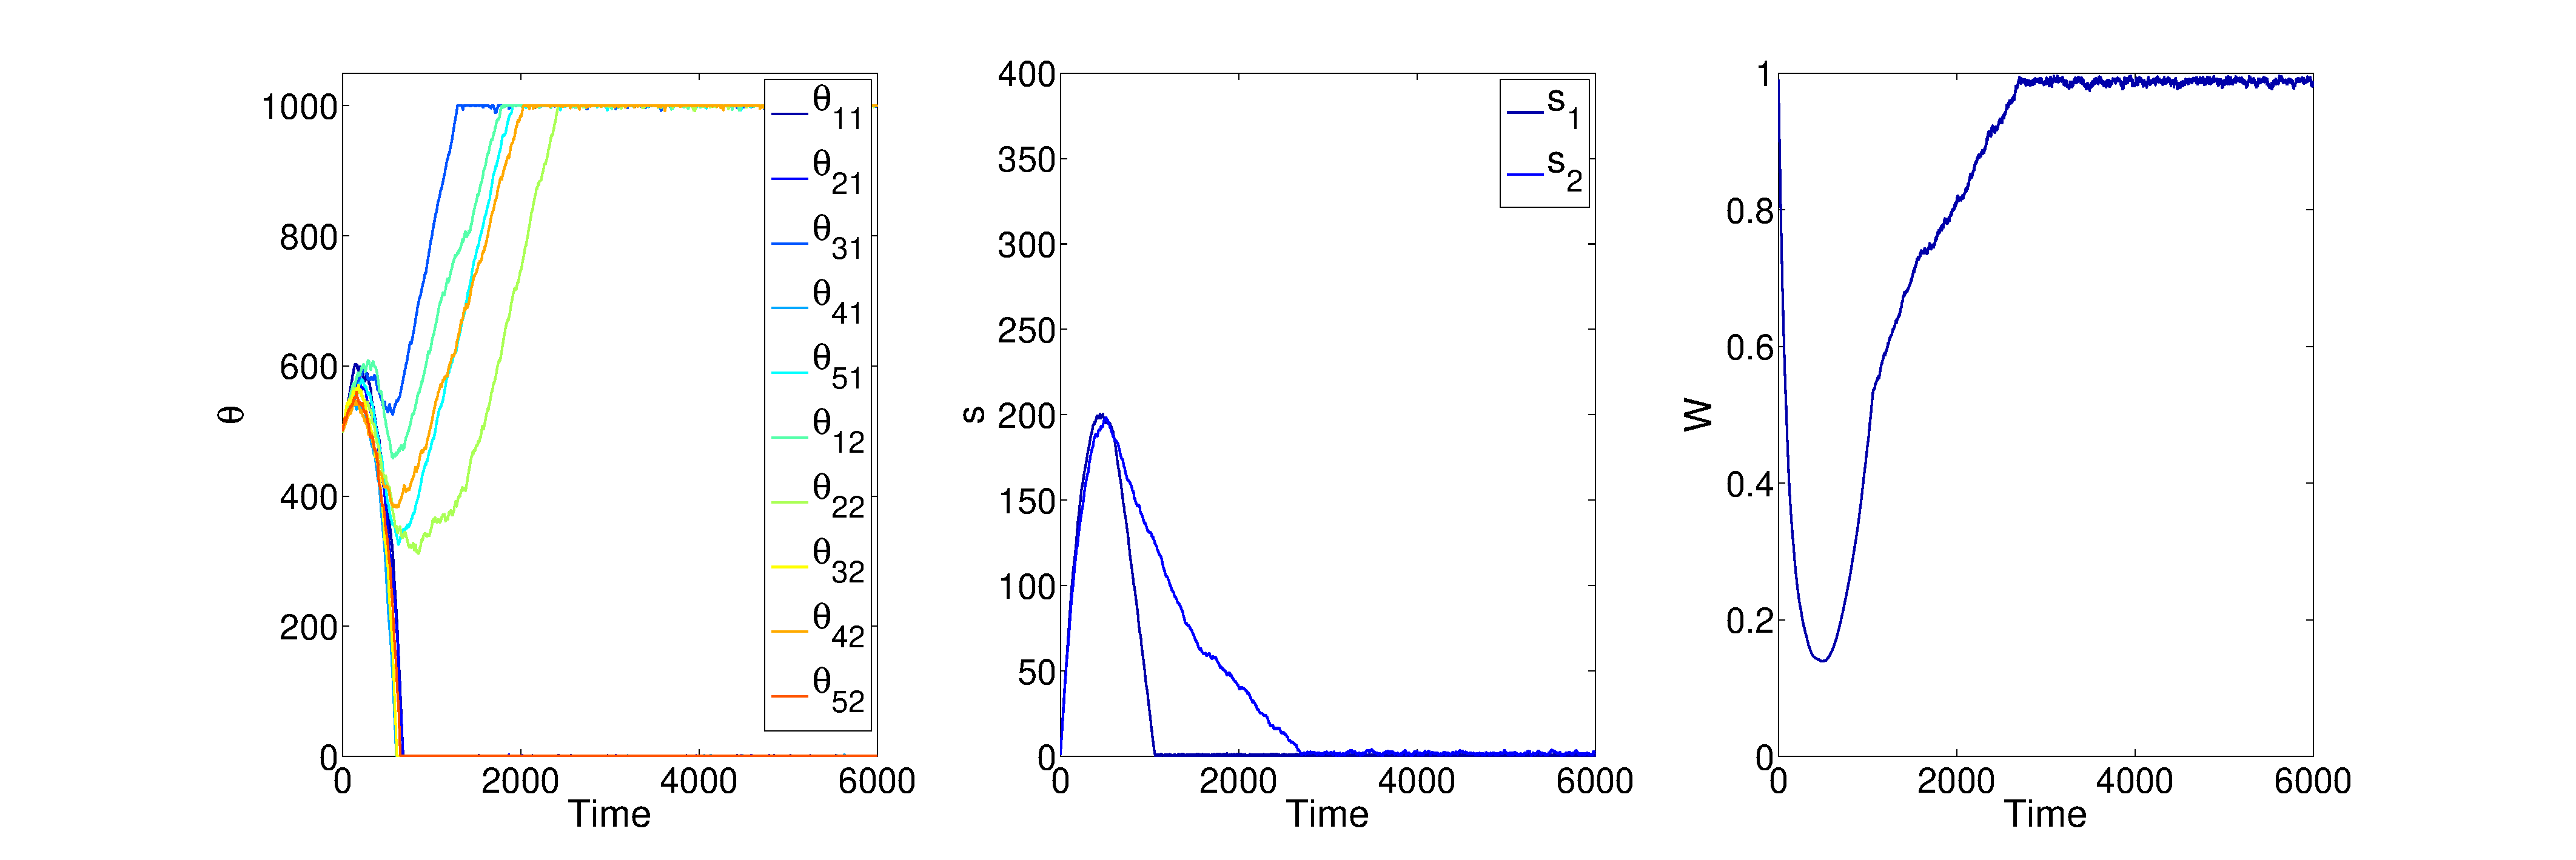
\includegraphics[width=1.25\textwidth]{../figures/welstim.eps}}
	
	\caption{Left: Tresholds $\theta$ as a function of time. Middle: Stimuli $s_{j}$ for task 1 and two as a function of time. Right: Welfare W as a function of time.}
	\label{fig:welstim}
\end{figure}

The functions can be interpreted as follows. The development of the stimuli can be explained by the fact that it takes time for the bees to reach an equilibrium state -- the state where all bees assume exactly one task. Up to this point, the needs of the hive are not sufficiently satisfied. Hence, the stimuli increase. Over time, the bees become more specialized towards a specific task and the stimuli go through a maximum to decrease subsequently. This is an expression that the tasks are performed with a sufficient efficiency. The individual development of the thresholds and stimuli is governed by how fast the bees manage to specialize themselves and satisfy the need for the respective task. In the presented case, for example, one can look at the stimulus and the threshold value which converge last to their equilibrium value - stimulus 2 and threshold $\theta_{22}$. Stimulus 2 decreases slower than stimulus 1, so the need to perform 2 is greater for a longer period of time compared to task 1. This is reflected in the curve of $\theta_{22}$. It remains low as long as stimulus 2 is high and only then converges to 1000. This means that bee 2 engages as long in task 2 as stimulus 2 remains high. Thereafter it becomes inactive with respect to task 2 and is thus the last bee to be fully specialized. The welfare is connected to the sum of the stimuli. The stimuli are high when the hive need that specific tasks need to be performed in order for the hive to survive. Whenever a task is not performed, or to an insufficient extent, the respective stimulus is high. High stimuli thus reflect a poor state. Vice versa, low stimuli show that the hive performs well. Therefore, we have introduced the welfare model which is based on the sum of the stimuli. When the sum of the stimuli is low, indicating a good performance of the hive, the welfare increases. Hence, our model is able to describe how well specific tasks are performed and to measure the total welfare of a population over time.


 

\subsection{PBM Model}
The PBM model is quite robust and a broad range of parameters deliver sensible results. Below we describe the influence of the more important parameters on time-dependant quantities such as allocated tasks, productivities, boredoms and salaries. 

Parameters for a standard simulation could be the following: $N=7$, $M=3$, $\lambda=0.01$, $\kappa=0.003$, $\zeta=0.001$, $\eta=0.0003$, $p_s=0.003$, $\Delta t=1$, $A_\mu=3$, $A_\sigma=0.7$, $P_\mu=2$, $P_\sigma=0.7$, $B_\mu=0.5$, $B_\sigma=0.15$. Figure~\ref{fig:sim1task} shows the time evolution of the tasks performed by the different workers. It allows to see the dynamics of work allocation. Figures~\ref{fig:sim1prod}, \ref{fig:sim1money} and \ref{fig:sim1boredom} allow to understand the motivation for choosing another task. Figure~\ref{fig:sim1prod} shows the evolution of the productivity at the current tasks and explains why workers performing the same task do not earn the same amount of money, which can be seen in Figure~\ref{fig:sim1money}. Figure~\ref{fig:sim1boredom} displays the evolution of the boredom. It illustrates that a too high boredom can induce a change of task even if the new task is less paid than the previous one. A general observation is that people working on tasks at which their maximam boredom is high tend to change the task rapidly because of the rapid increase of the boredom. Figure~\ref{fig:sim1totalmoney} shows the total amount of money earned so far by each of the workers. It features a pronounced social inequality, which is caused by two main factors. Firstly, the inherent characteristics of the workers make some of them much more productive, thence earning more money. The second factor has its origin in the society, more precisely in the production of other individuals; it could be illustrated by the fact that a not particularly skilled individual will be remunerated a lot if he is the only one able to do his job, while two very skilled individuals at the same task will earn much less.

\begin{figure}[hp!]
	\centering
	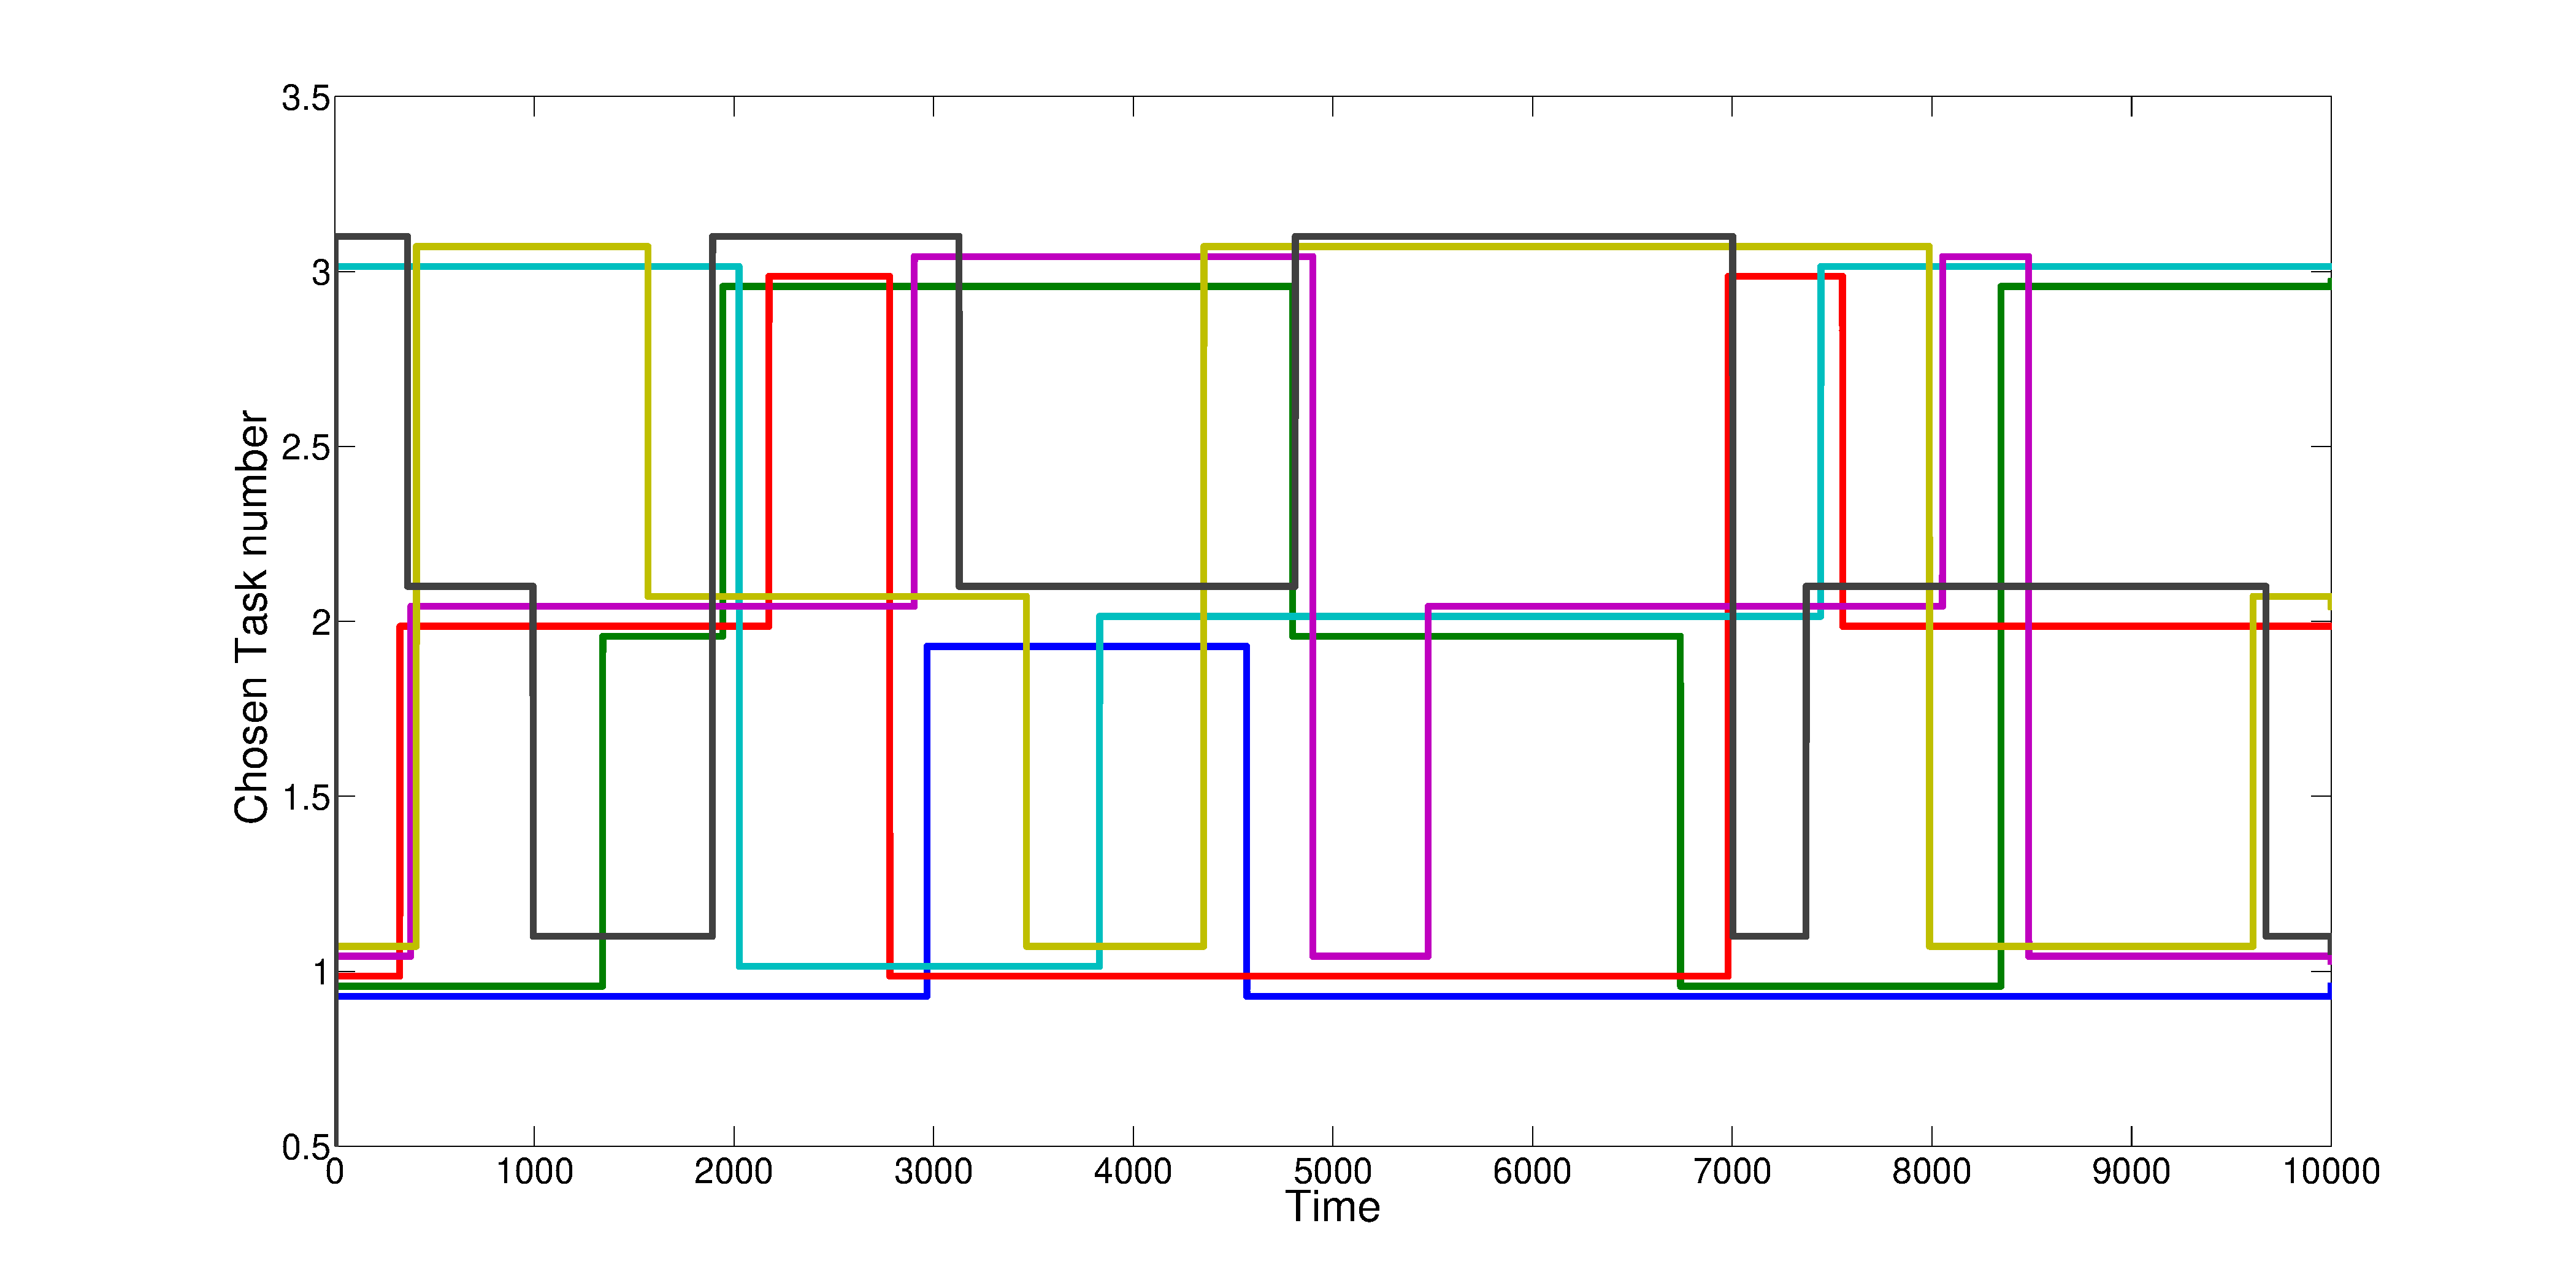
\includegraphics[width=0.9\textwidth]{../figures/taskno.pdf}
	\caption{Current tasks of the workers as a function of time. Each worker is represented by a different color. The curves of the different individui have a small vertical shift so that all the lines are visible.}
	\label{fig:sim1task}
\end{figure}

\begin{figure}[hp!]
	\centering
	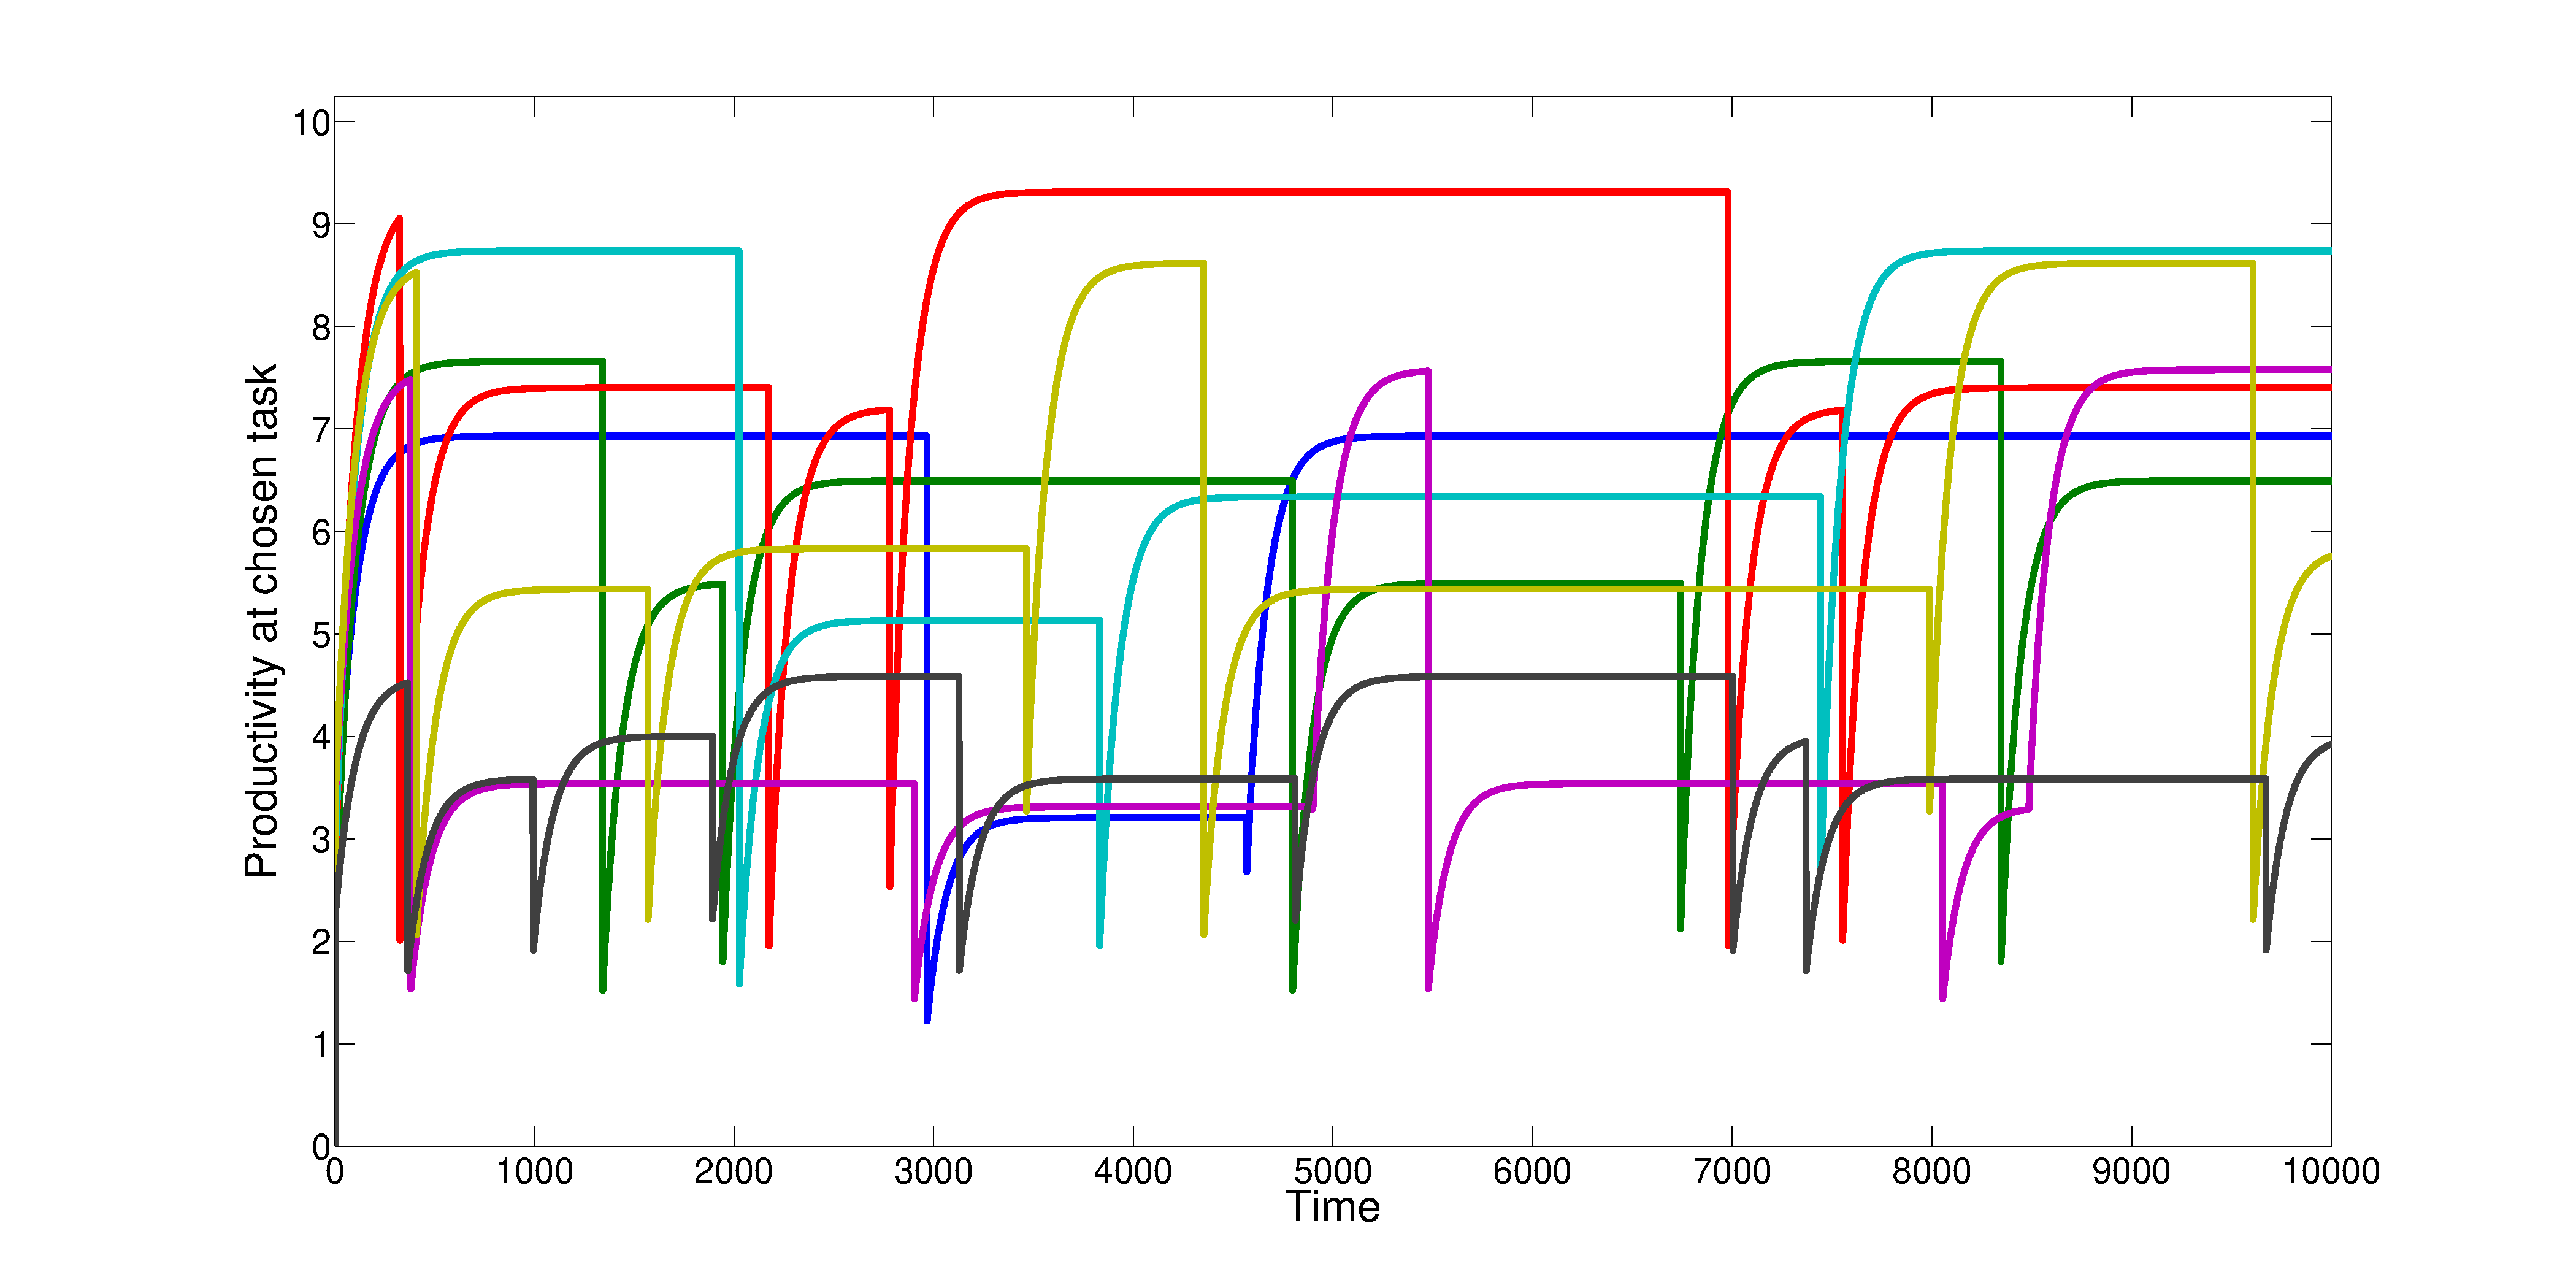
\includegraphics[width=0.9\textwidth]{../figures/productivity.pdf}
	\caption{Productivity of the workers at the tasks they are currently performing. The incontinuities mark a change in the task and correspond to what is shown in Figure~\ref{fig:sim1task}.}
	\label{fig:sim1prod}
\end{figure}

\begin{figure}[hp!]
	\centering
	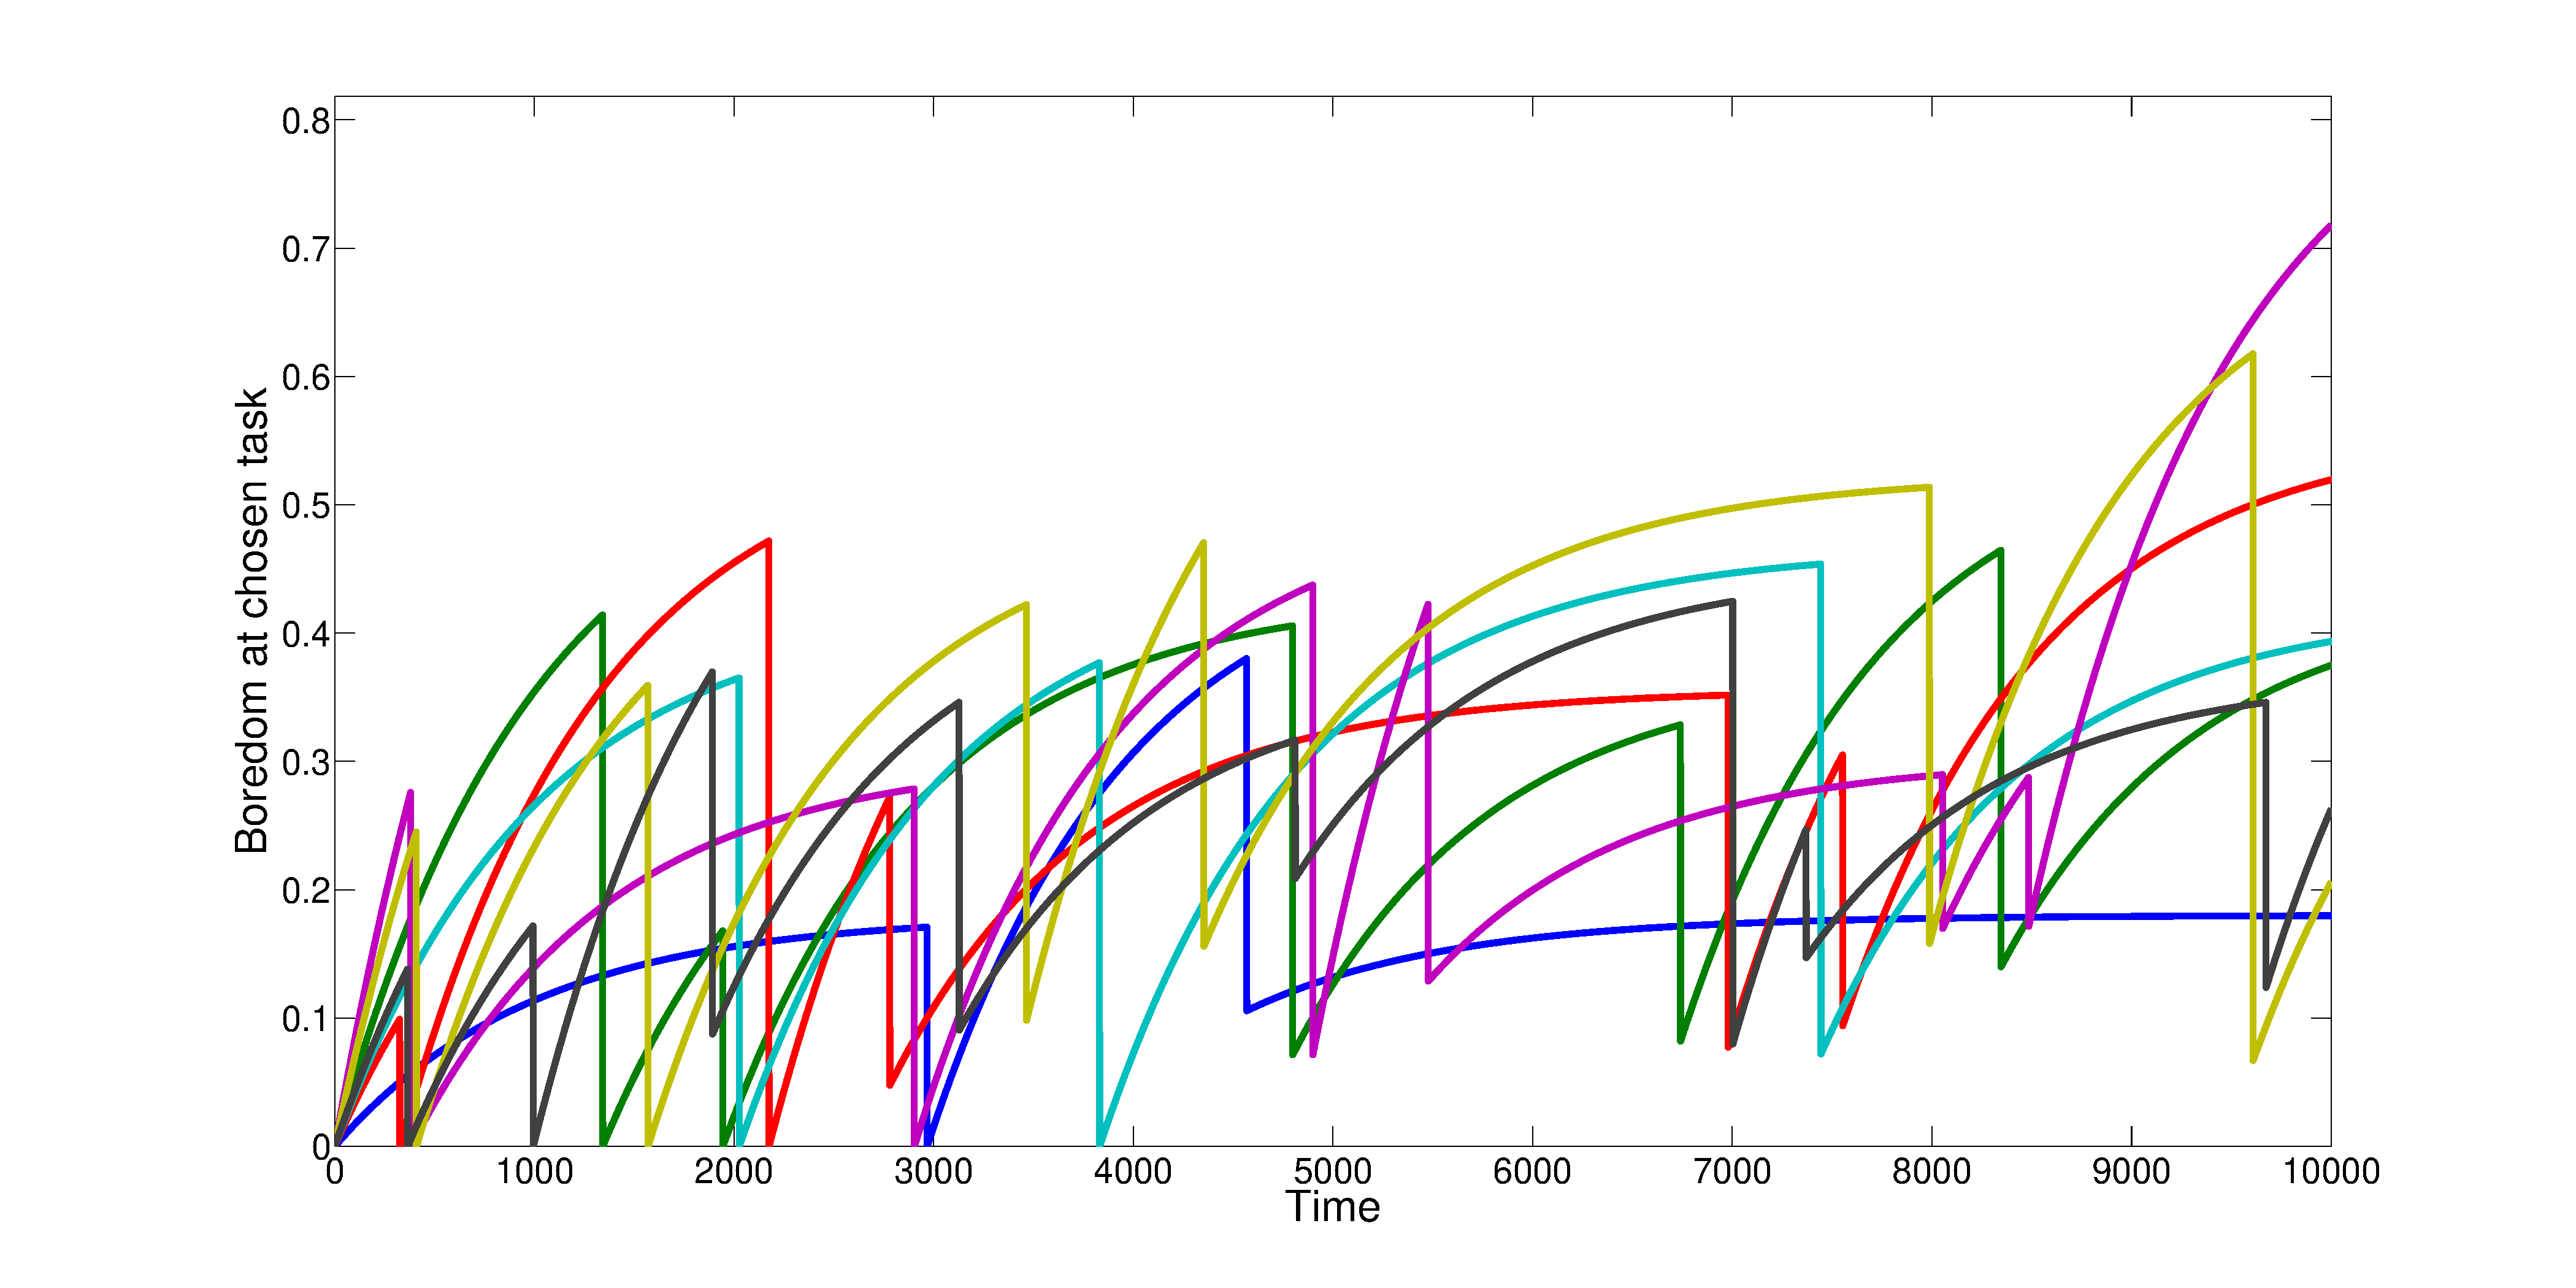
\includegraphics[width=0.9\textwidth]{../figures/boredom.pdf}
	\caption{Boredom of the workers at the tasks they are currently performing. It can be seen that the maximal boredom is not achieved in most of the cases, since the boredom becomes too high.}
	\label{fig:sim1boredom}
\end{figure}

\begin{figure}[hp!]
	\centering
	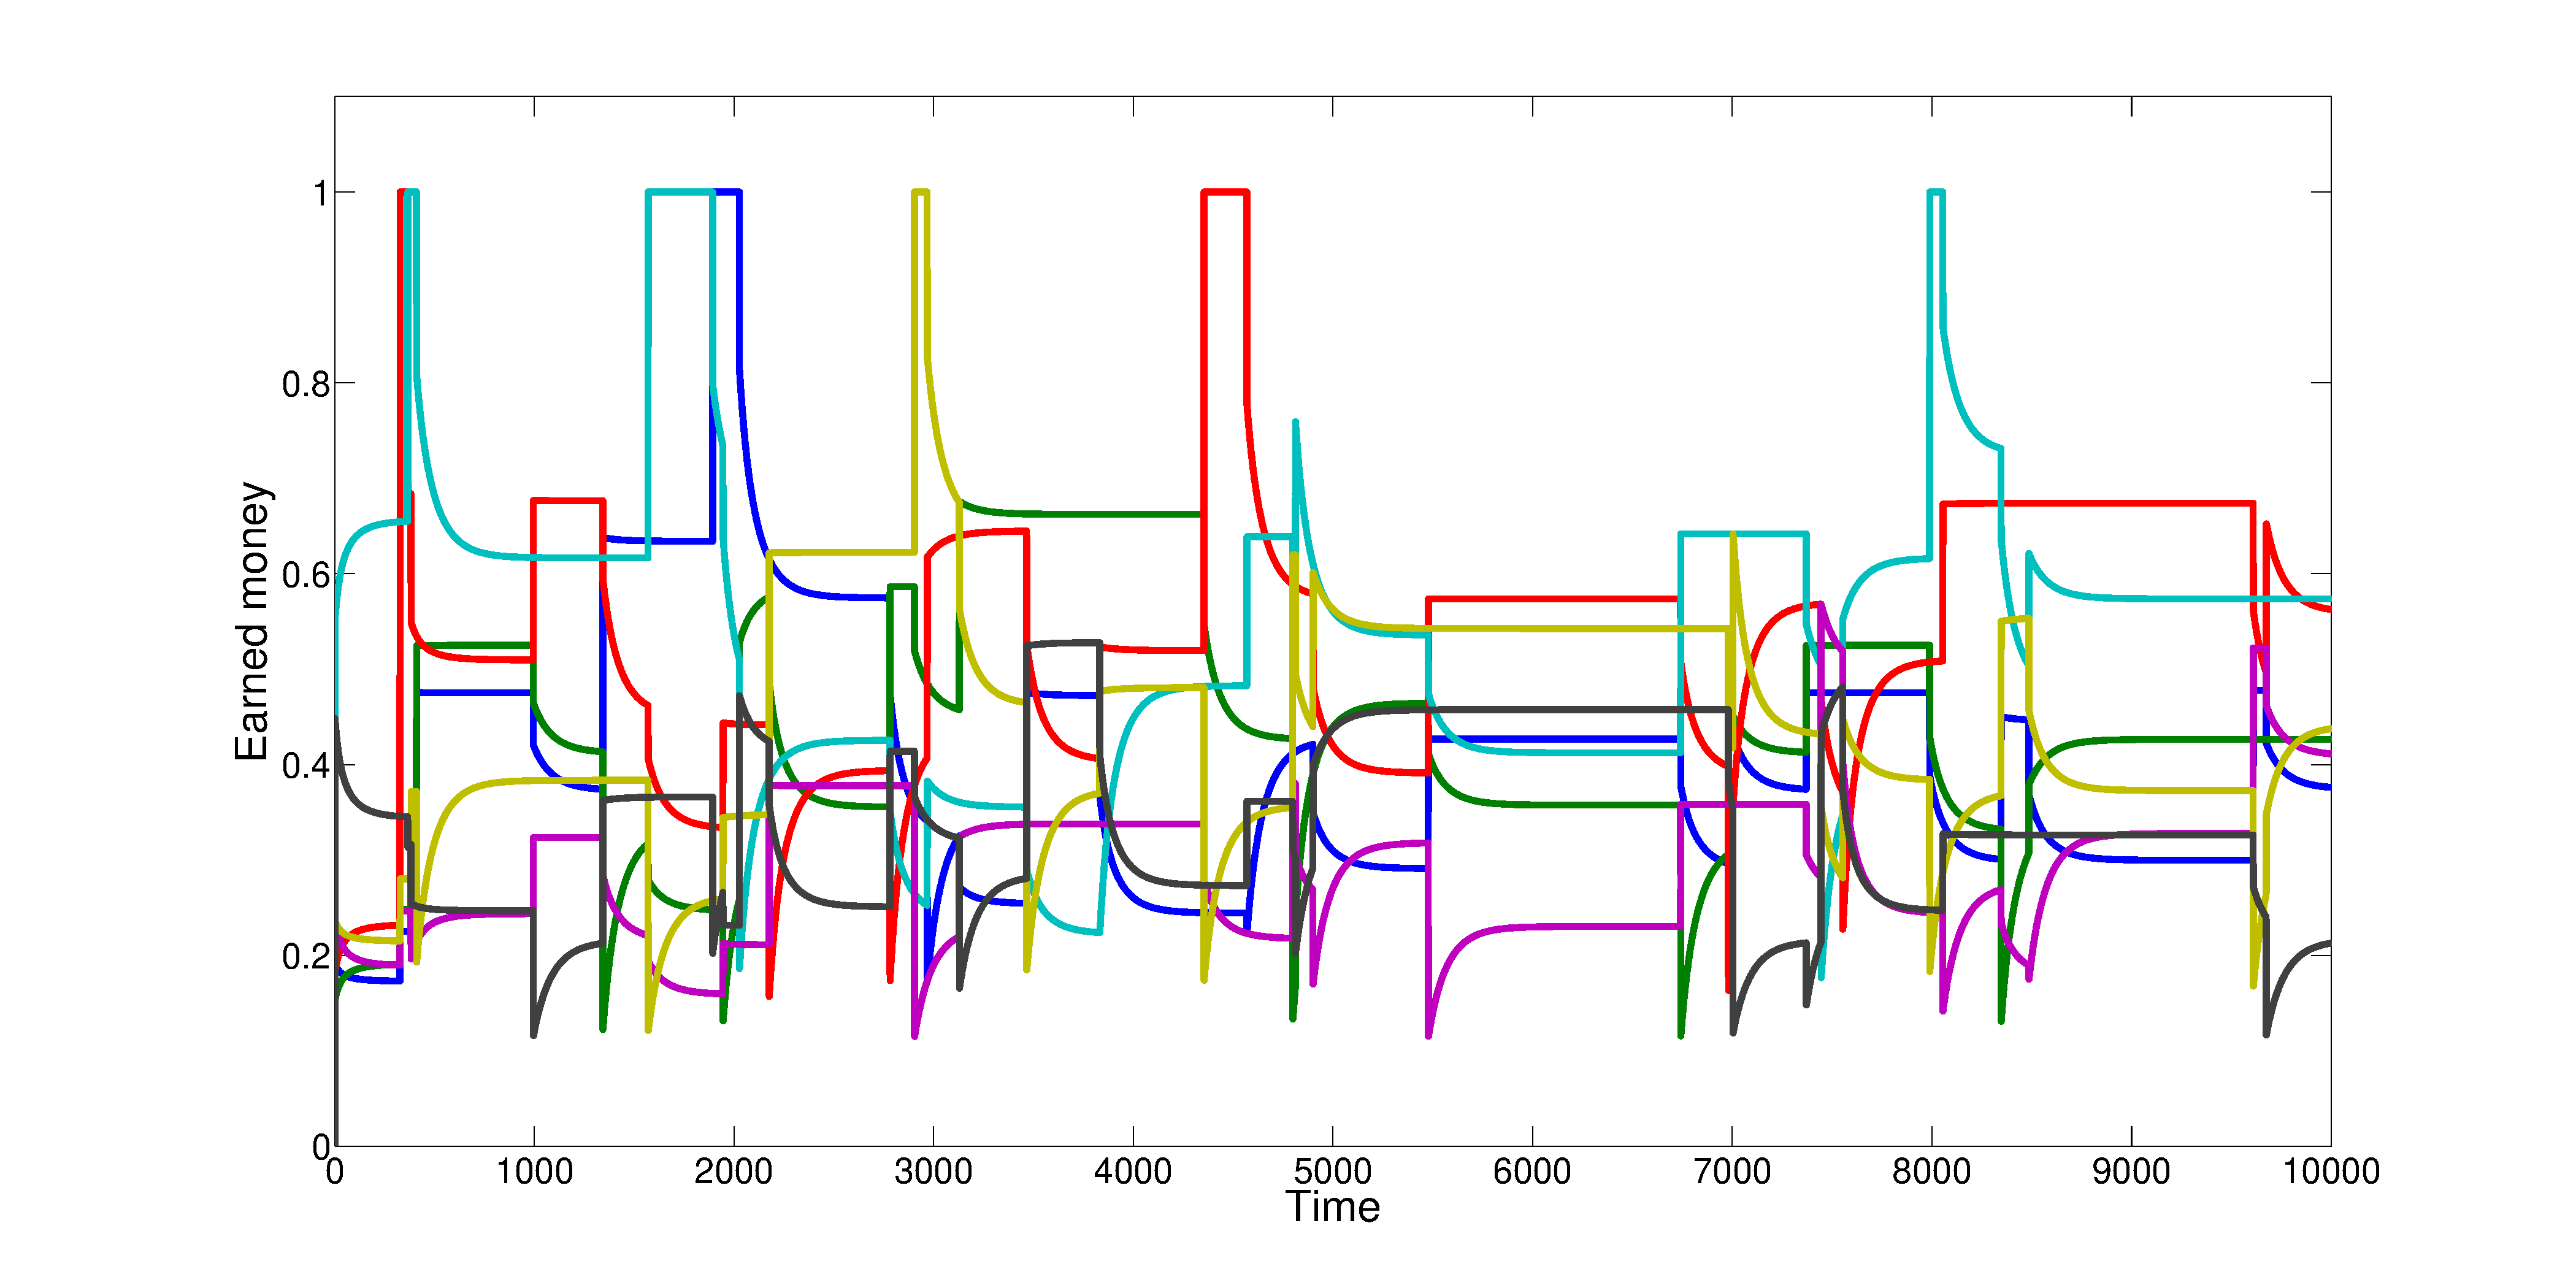
\includegraphics[width=0.9\textwidth]{../figures/money.pdf}
	\caption{Salary of the workers as a function of time. A salary of 1 means that a worker is the only one to perform his current task and therefore gets all the money granted to the task.}
	\label{fig:sim1money}
\end{figure}

\begin{figure}[hp!]
	\centering
	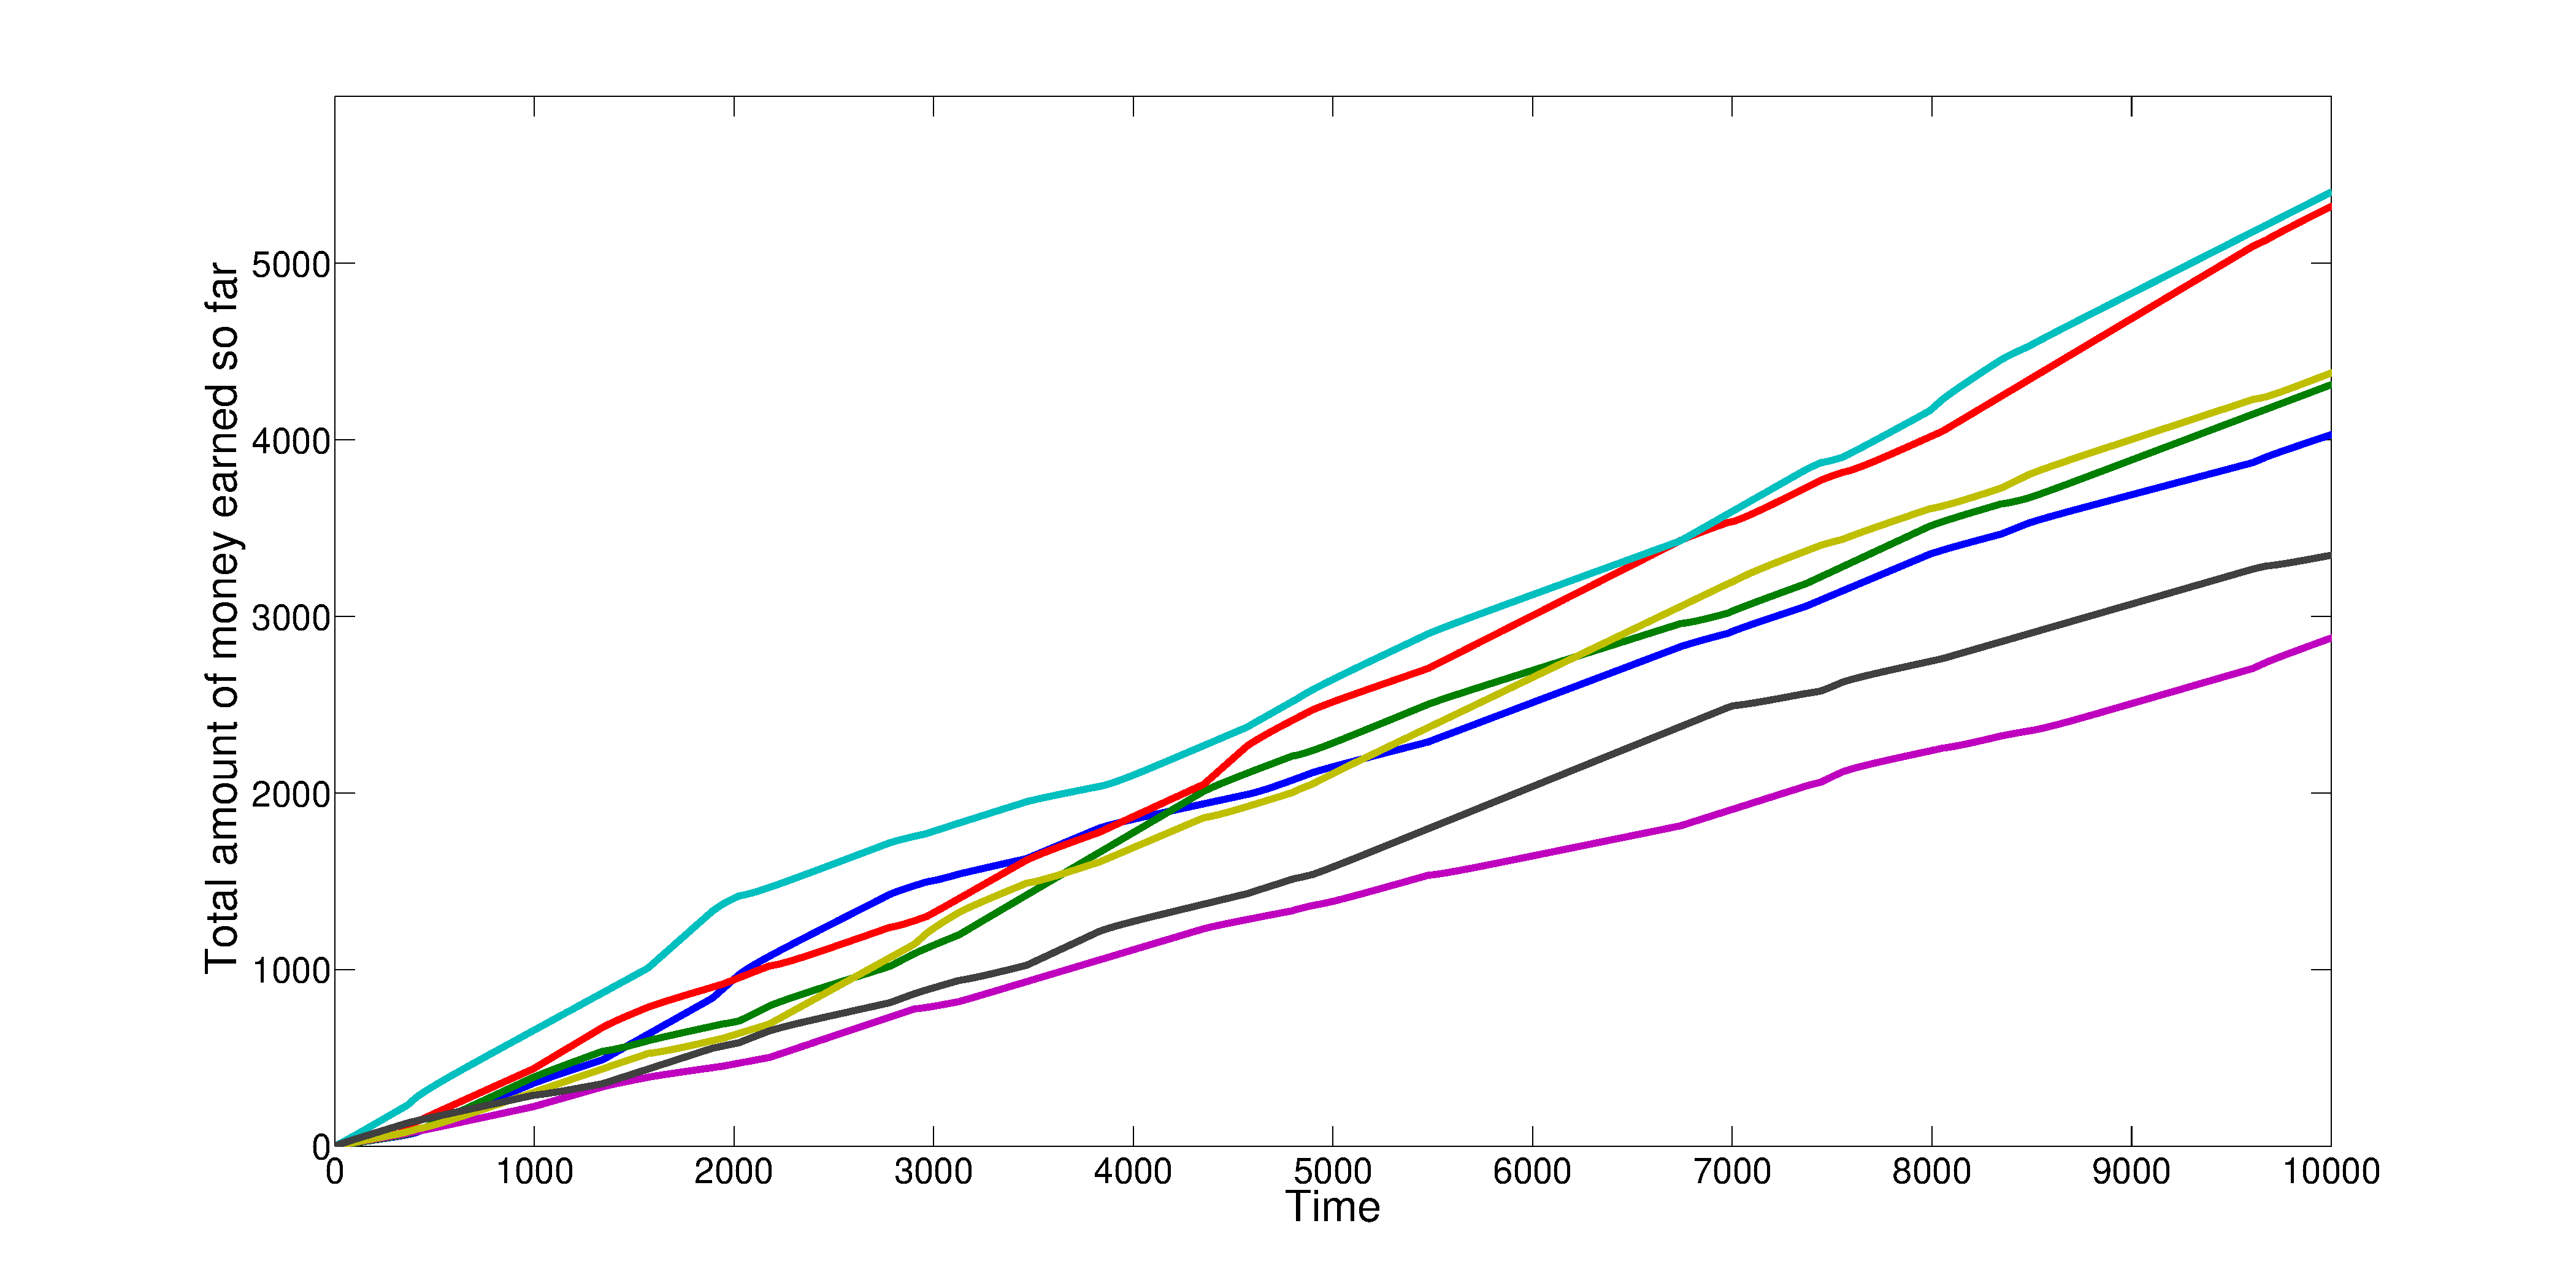
\includegraphics[width=0.9\textwidth]{../figures/totalmoney.pdf}
	\caption{Total money earned by each of the workers. It illustrates how the social inequalities are steadily increasing, and the hierarchy of the society stays the same over during the simulation.}
	\label{fig:sim1totalmoney}
\end{figure}

The randomness used in generation of the productivities $P_{ij}$ and of the abilities $A_i$ allow the inspection of social inequality. Both quantities have a similar influence, with the difference that the differences in $P_{ij}$ are both task- and worker-specific, while the differences in $A_i$ are worker-specific. Setting the standard deviation of the distributions to zero would result in a model with much less social inequality, which is not the scope of the present model. The larger the standard deviation, the more pronounced the social inequalities will be. Figures~\ref{fig:sd1} and \ref{fig:sd2} illustrate the influence of the standard deviation used for the generation of the abilities and the initial productivities on social inequality.

\begin{figure}[hp!]
	\centering
	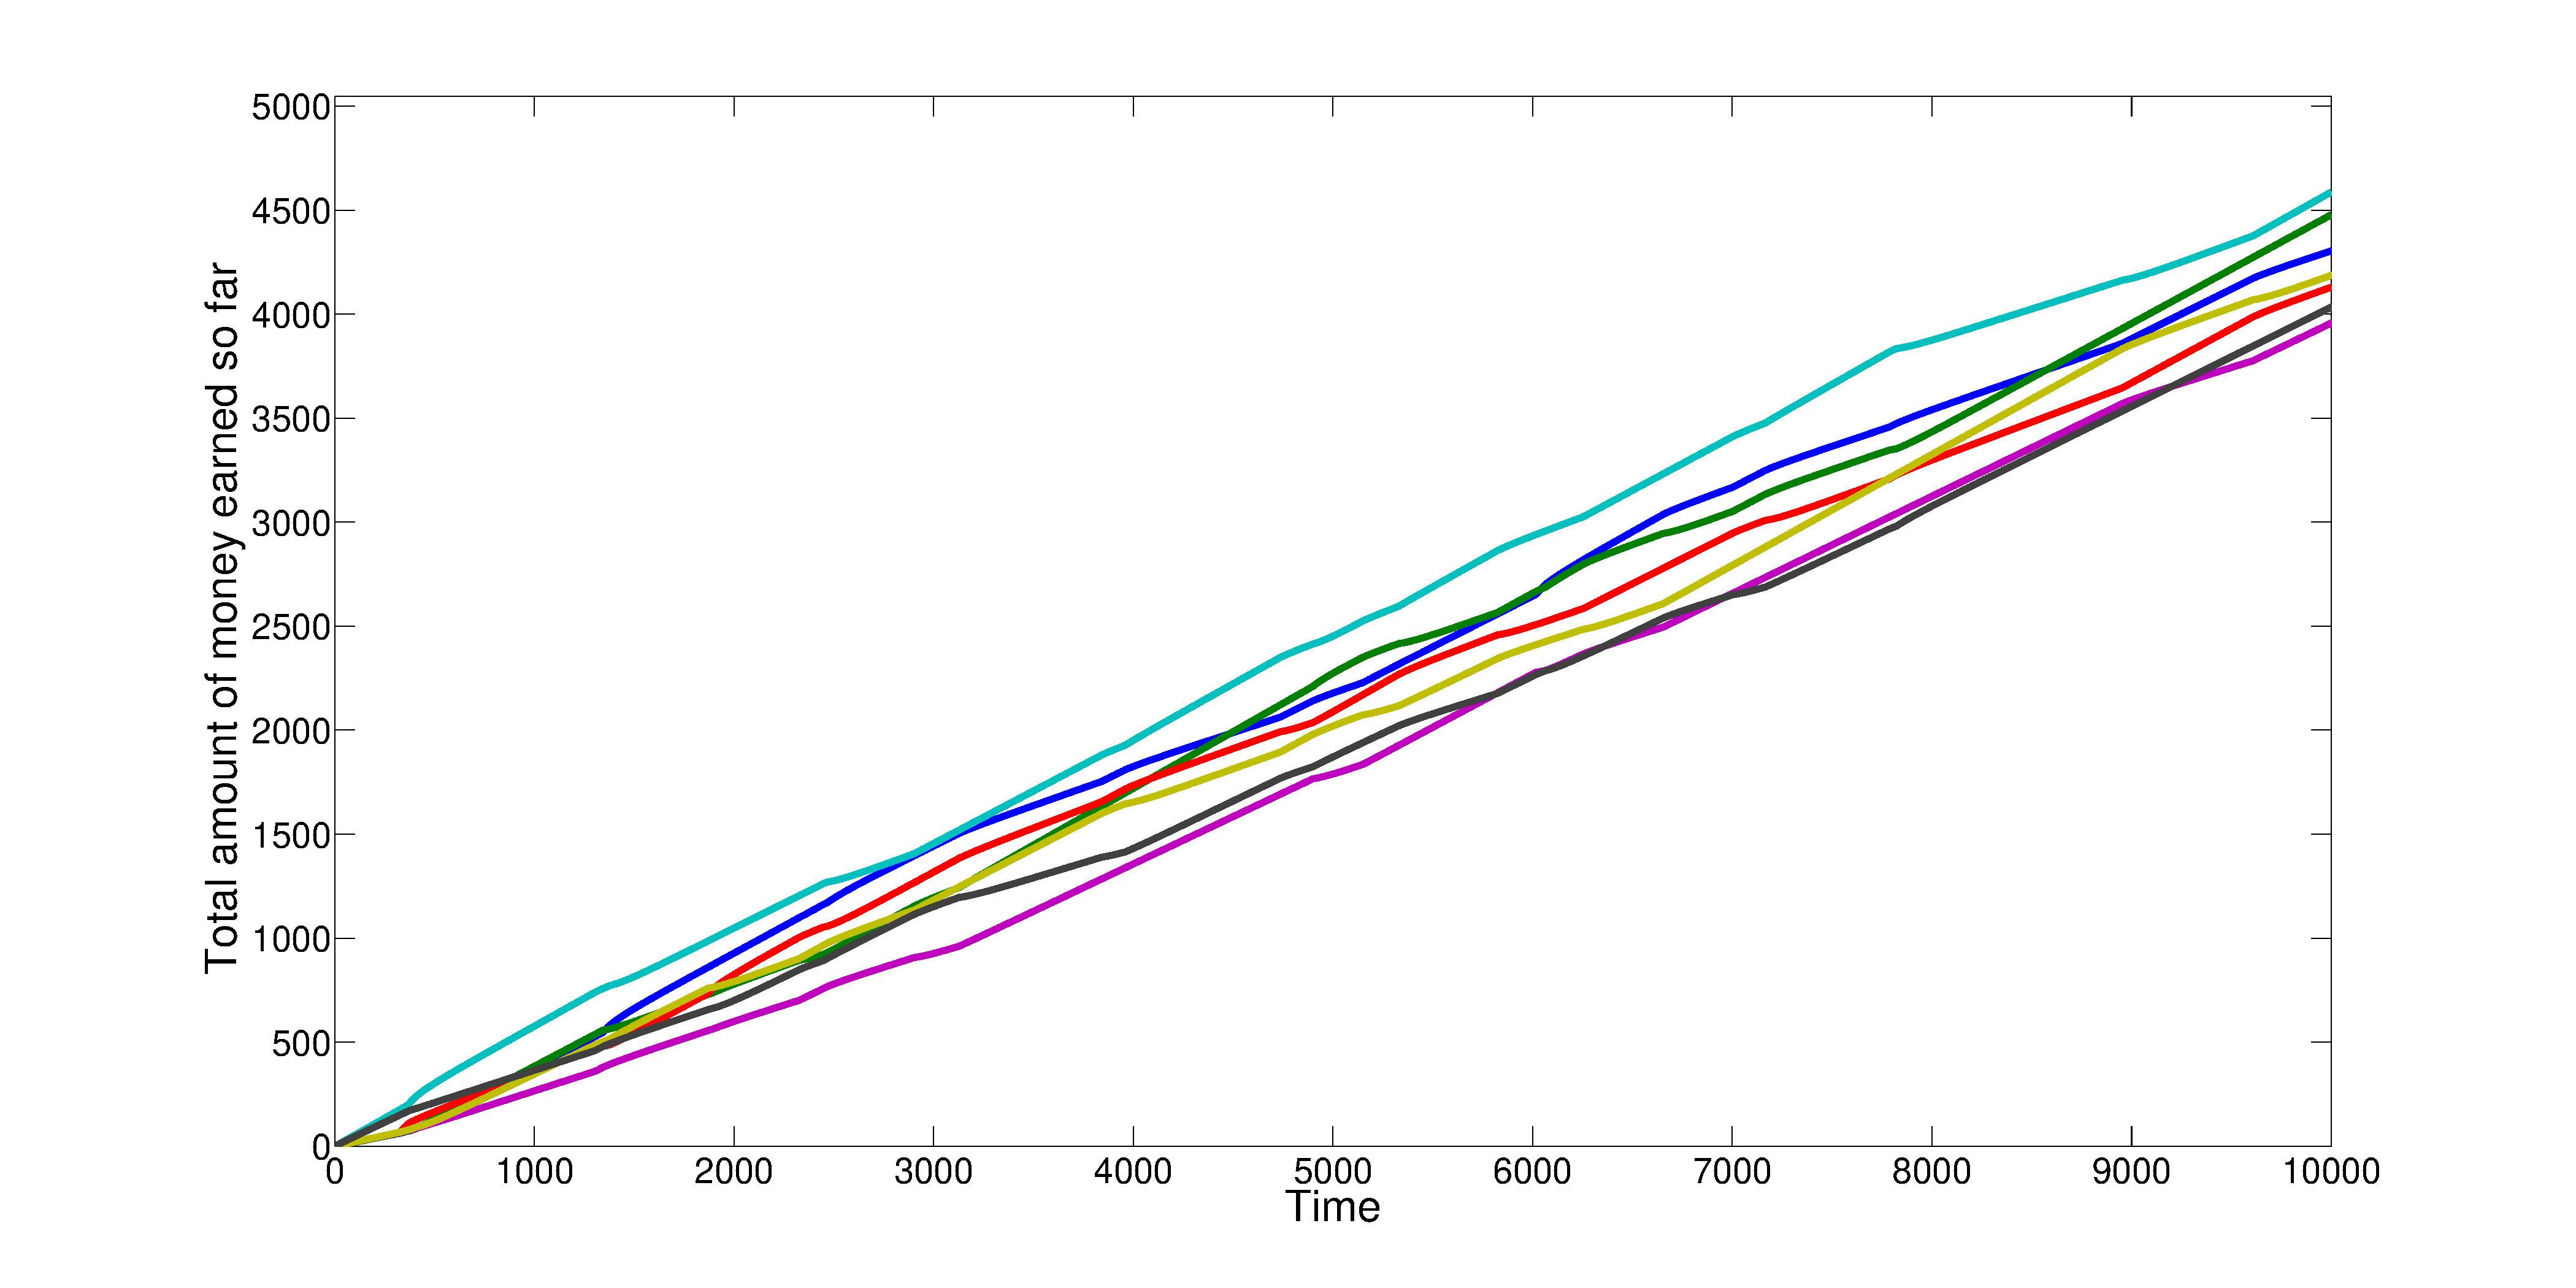
\includegraphics[width=0.9\textwidth]{../figures/sd1.pdf}
	\caption{Total money earned by each of the workers. But for $P_\sigma=0.2$ and $A_\sigma=0.2$, the same parameters as in Figure~\ref{fig:sim1totalmoney} were used. The social inequalities remain narrow and do not increase a lot with time.}
	\label{fig:sd1}
\end{figure}

\begin{figure}[hp!]
	\centering
	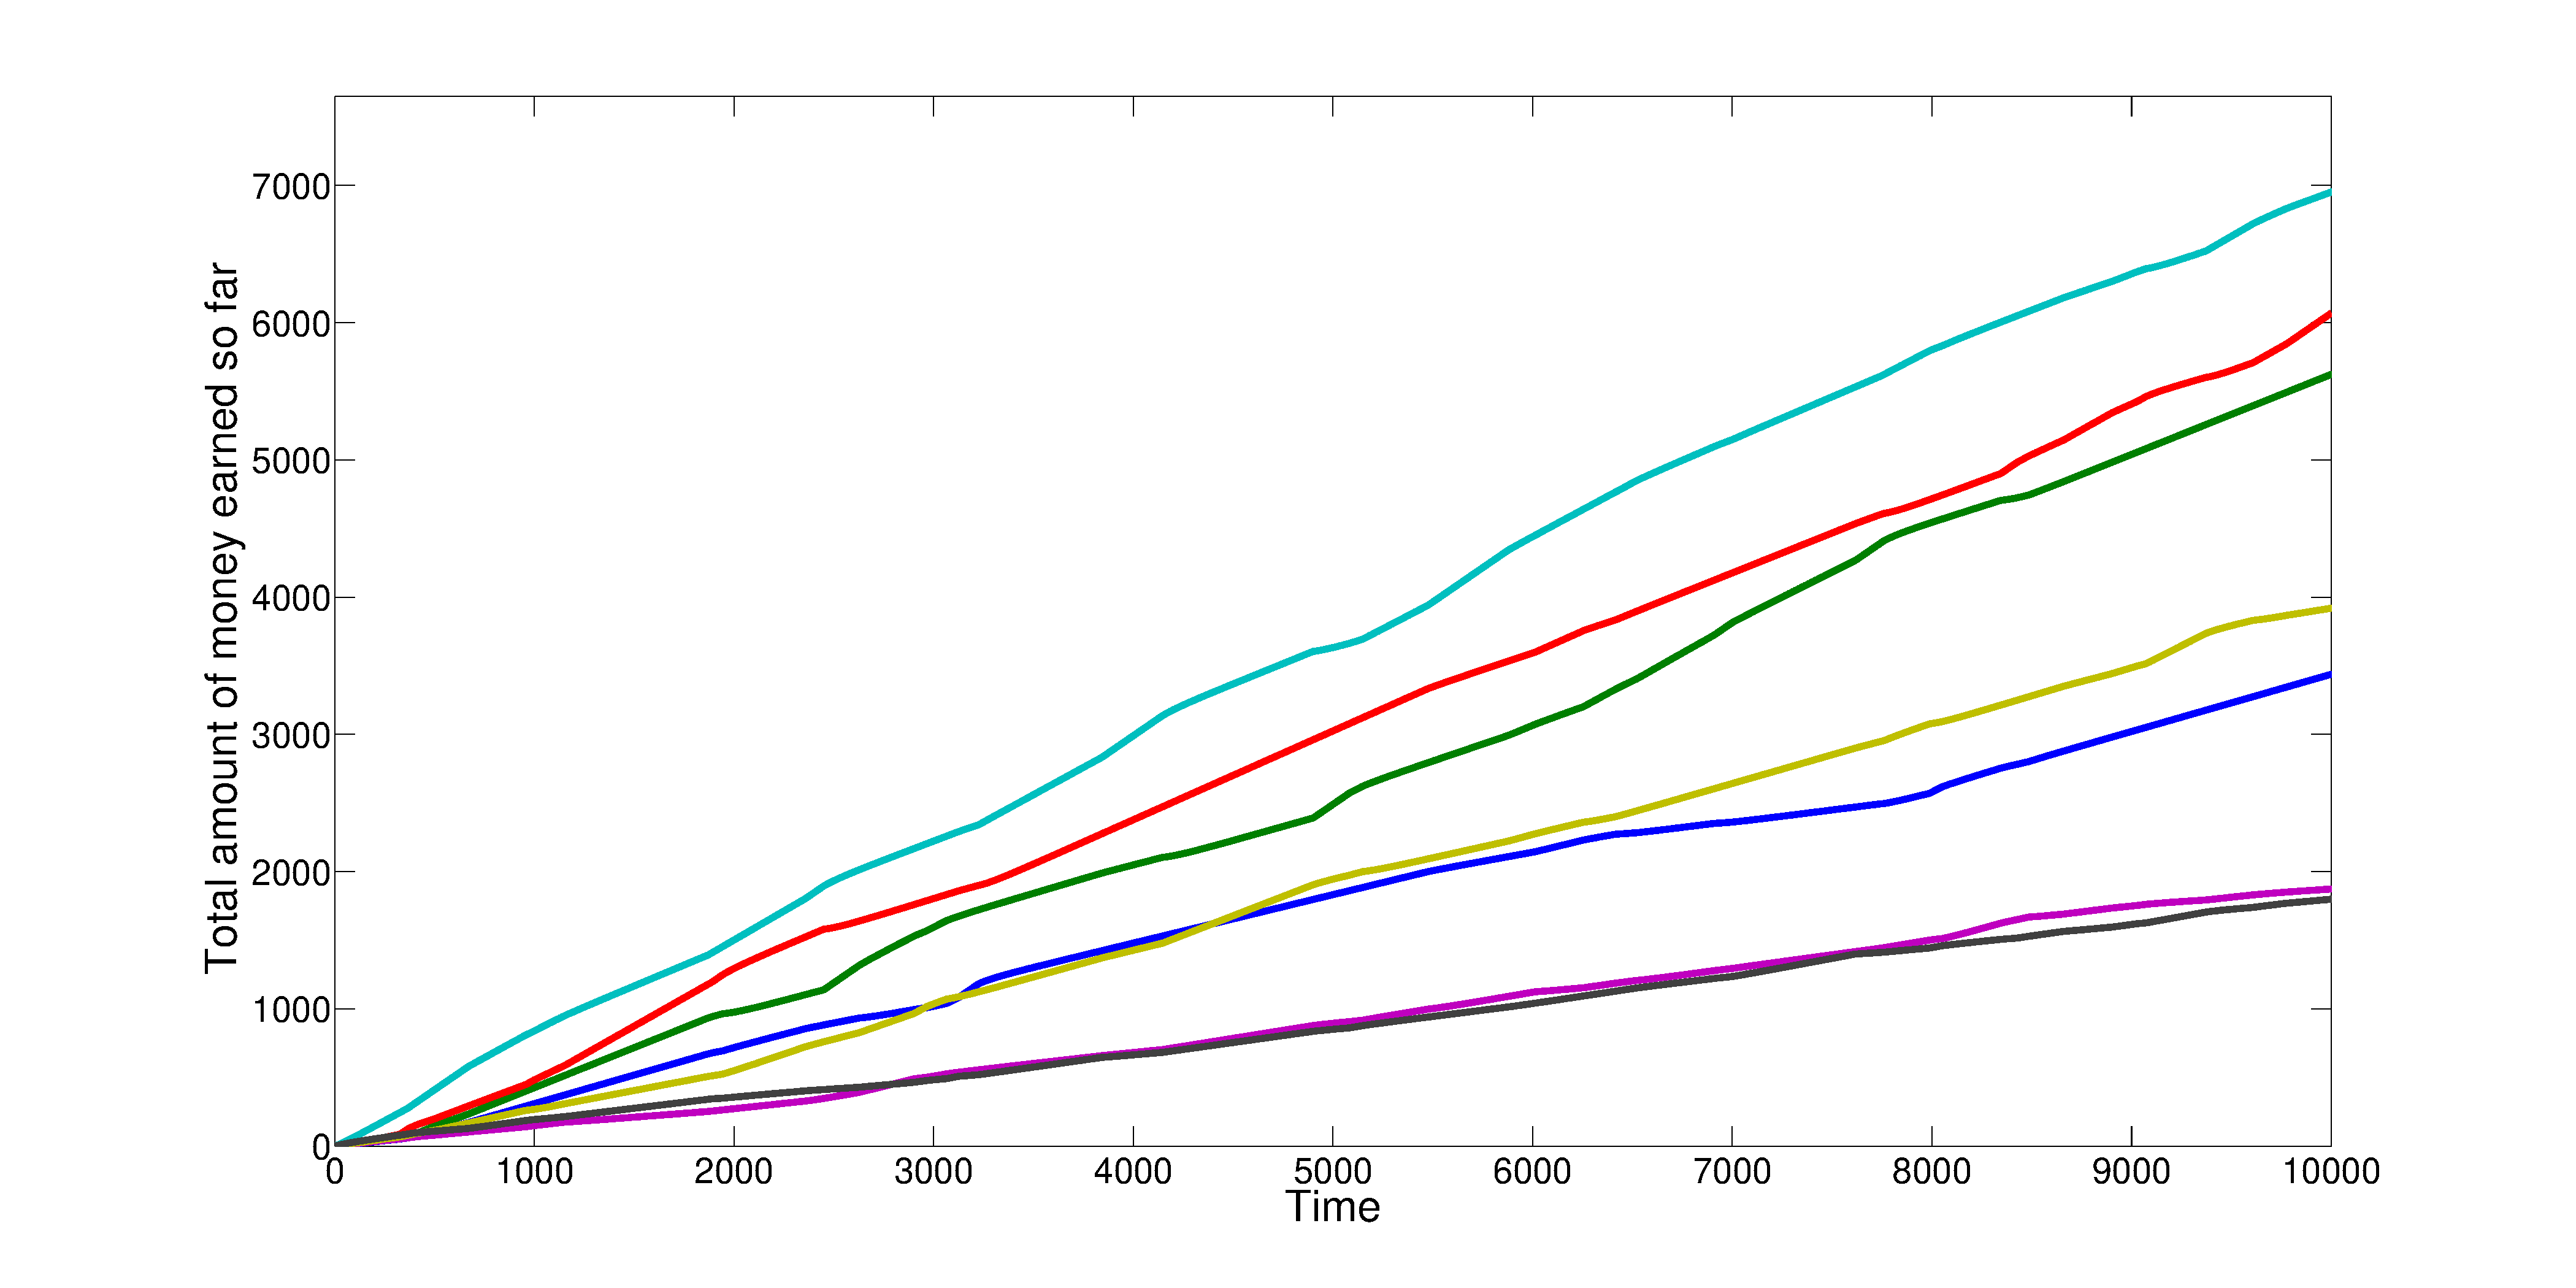
\includegraphics[width=0.9\textwidth]{../figures/sd2.pdf}
	\caption{Total money earned by each of the workers. But for $P_\sigma=1.0$ and $A_\sigma=1.4$, the same parameters as in Figure~\ref{fig:sim1totalmoney} were used. The social gap increases a lot and some workers earn several times the salary of other individui.}
	\label{fig:sd2}
\end{figure}
The boredom can be seen as the main reason for choosing a new task. Figure~\ref{fig:noboredom} was obtained by using $\zeta=0$ instead of $\zeta=0.001$ as above. It displays a prompt work specialization, illustrated by the fact that after a short equilibration period, there are no more task changes due to the absence of boredom. 
Figure~\ref{fig:moreboredom1} and \ref{fig:moreboredom2}, on the other hand, were obtained with $\zeta=0.01$ and $B_\mu=1.5$. They show the more frequent task changes and the higher average boredom. It is to be noted that the high sensitivity to boredom in this case does not diminish the social inequalities, which can be seen in Figure~\ref{fig:moreboredom3}. 

The randomness in the generation of $B_{ij}^\textrm{max}$ allows the differenciated sensibility to boredom, which, as mentioned above, has an influence on the rate at which an individual will change tasks.

Another cause for a change in the task is the evolution of the market, meaning that a worker is more likely to leave his current task if a new individuum just joined the new task, thus lowering the average salary.

\begin{figure}[hp!]
	\centering
	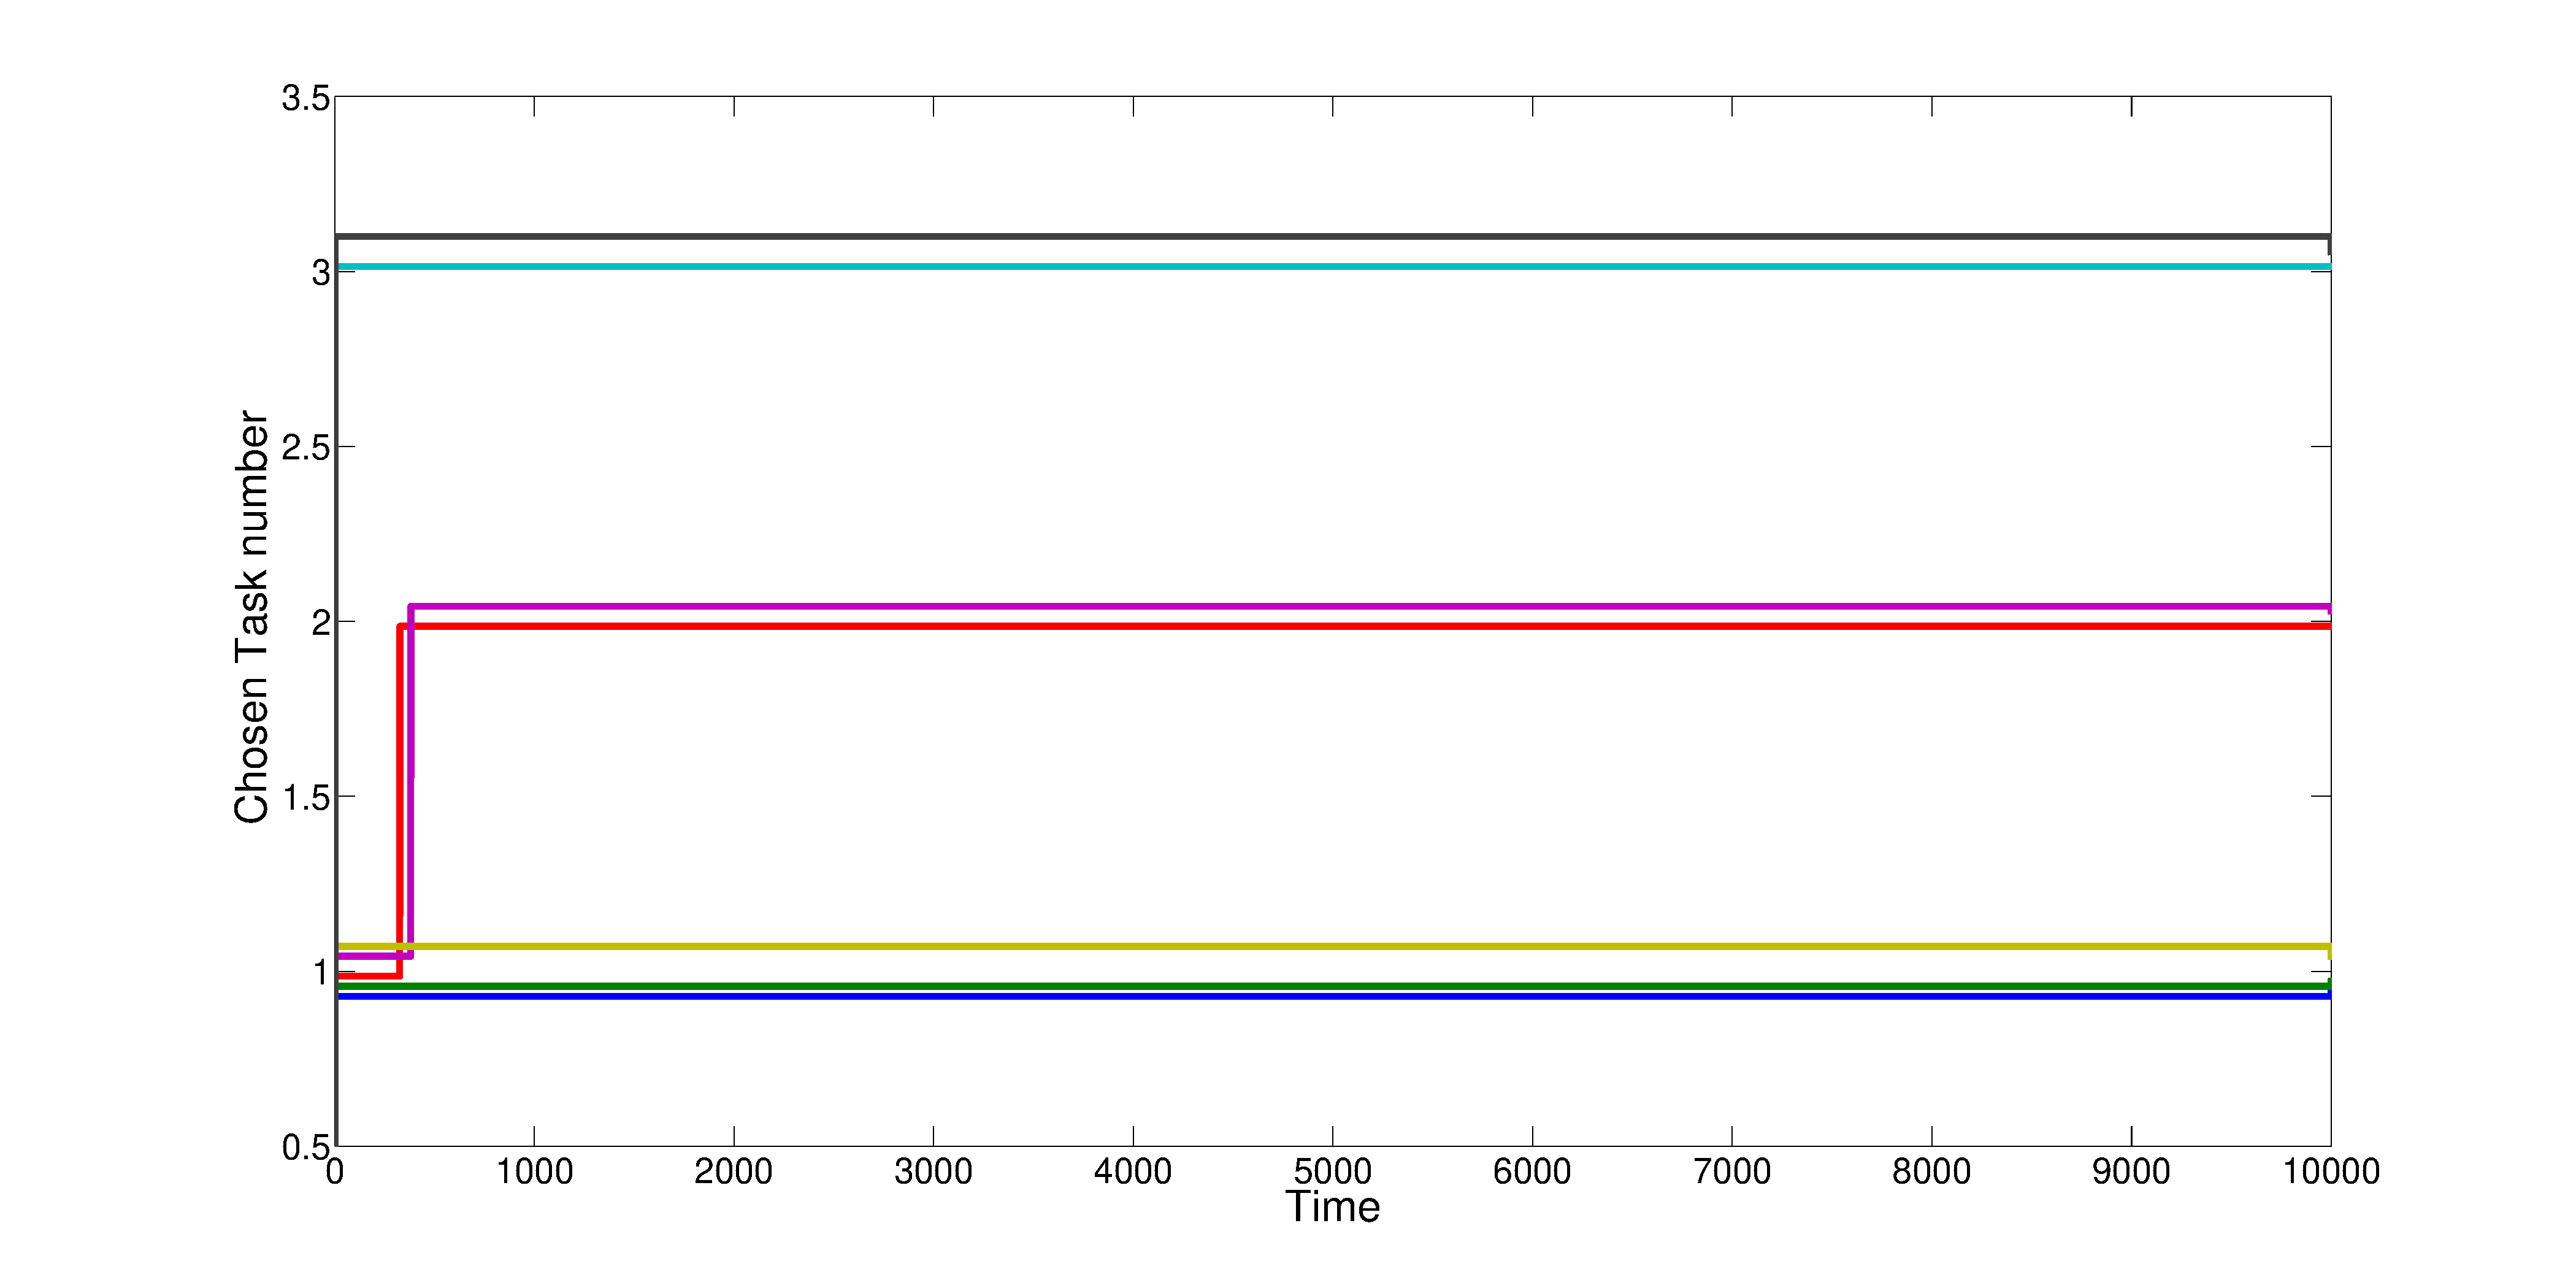
\includegraphics[width=0.9\textwidth]{../figures/noboredom.pdf}
	\caption{Chosen task number as a function of time. The same parameters as in Figure~\ref{fig:sim1task} were used but for $\zeta=0$, which implies that the workers do not experience any boredom at all. It shows an early change of task for two of the workers, after which the system does not change anymore.}
	\label{fig:noboredom}
\end{figure}

\begin{figure}[hp!]
	\centering
	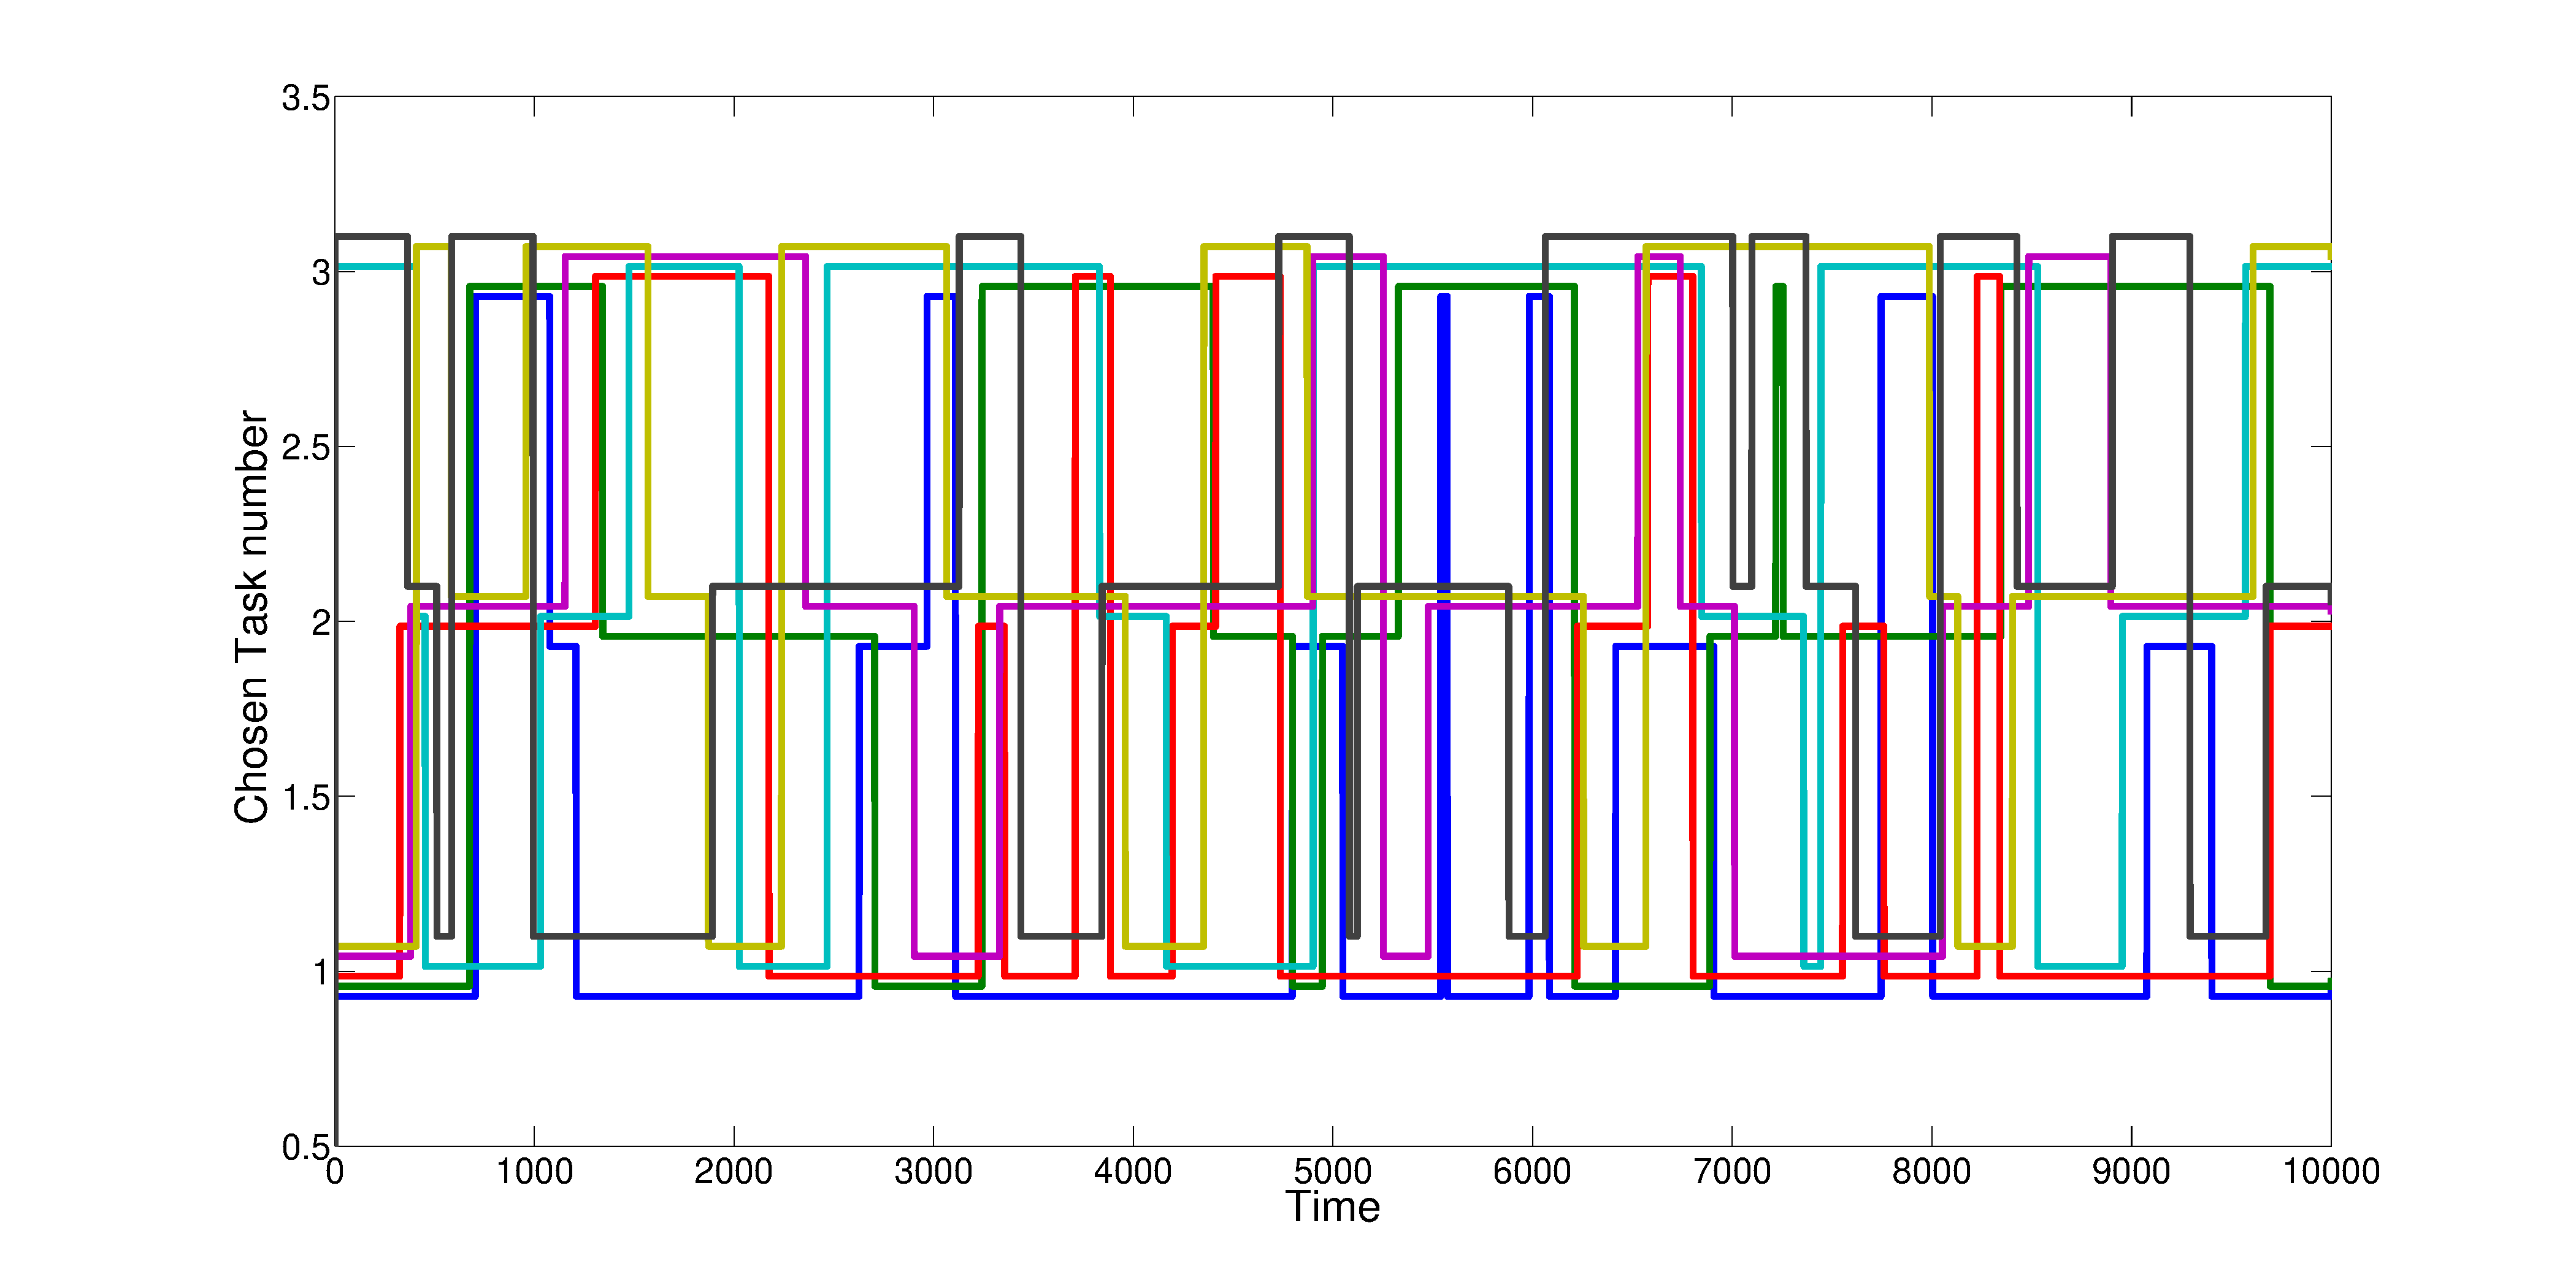
\includegraphics[width=0.9\textwidth]{../figures/moreboredom1.pdf}
	\caption{Chosen task number with $\zeta=0.01$ and $B_\mu=1.5$. All the other parameters are the same ones as used for Figure~\ref{fig:sim1task}. The very high rate of task changes is mainly due to the high average boredom, which is displayed in Figure~\ref{fig:moreboredom2}.}
	\label{fig:moreboredom1}
\end{figure}

\begin{figure}[hp!]
	\centering
	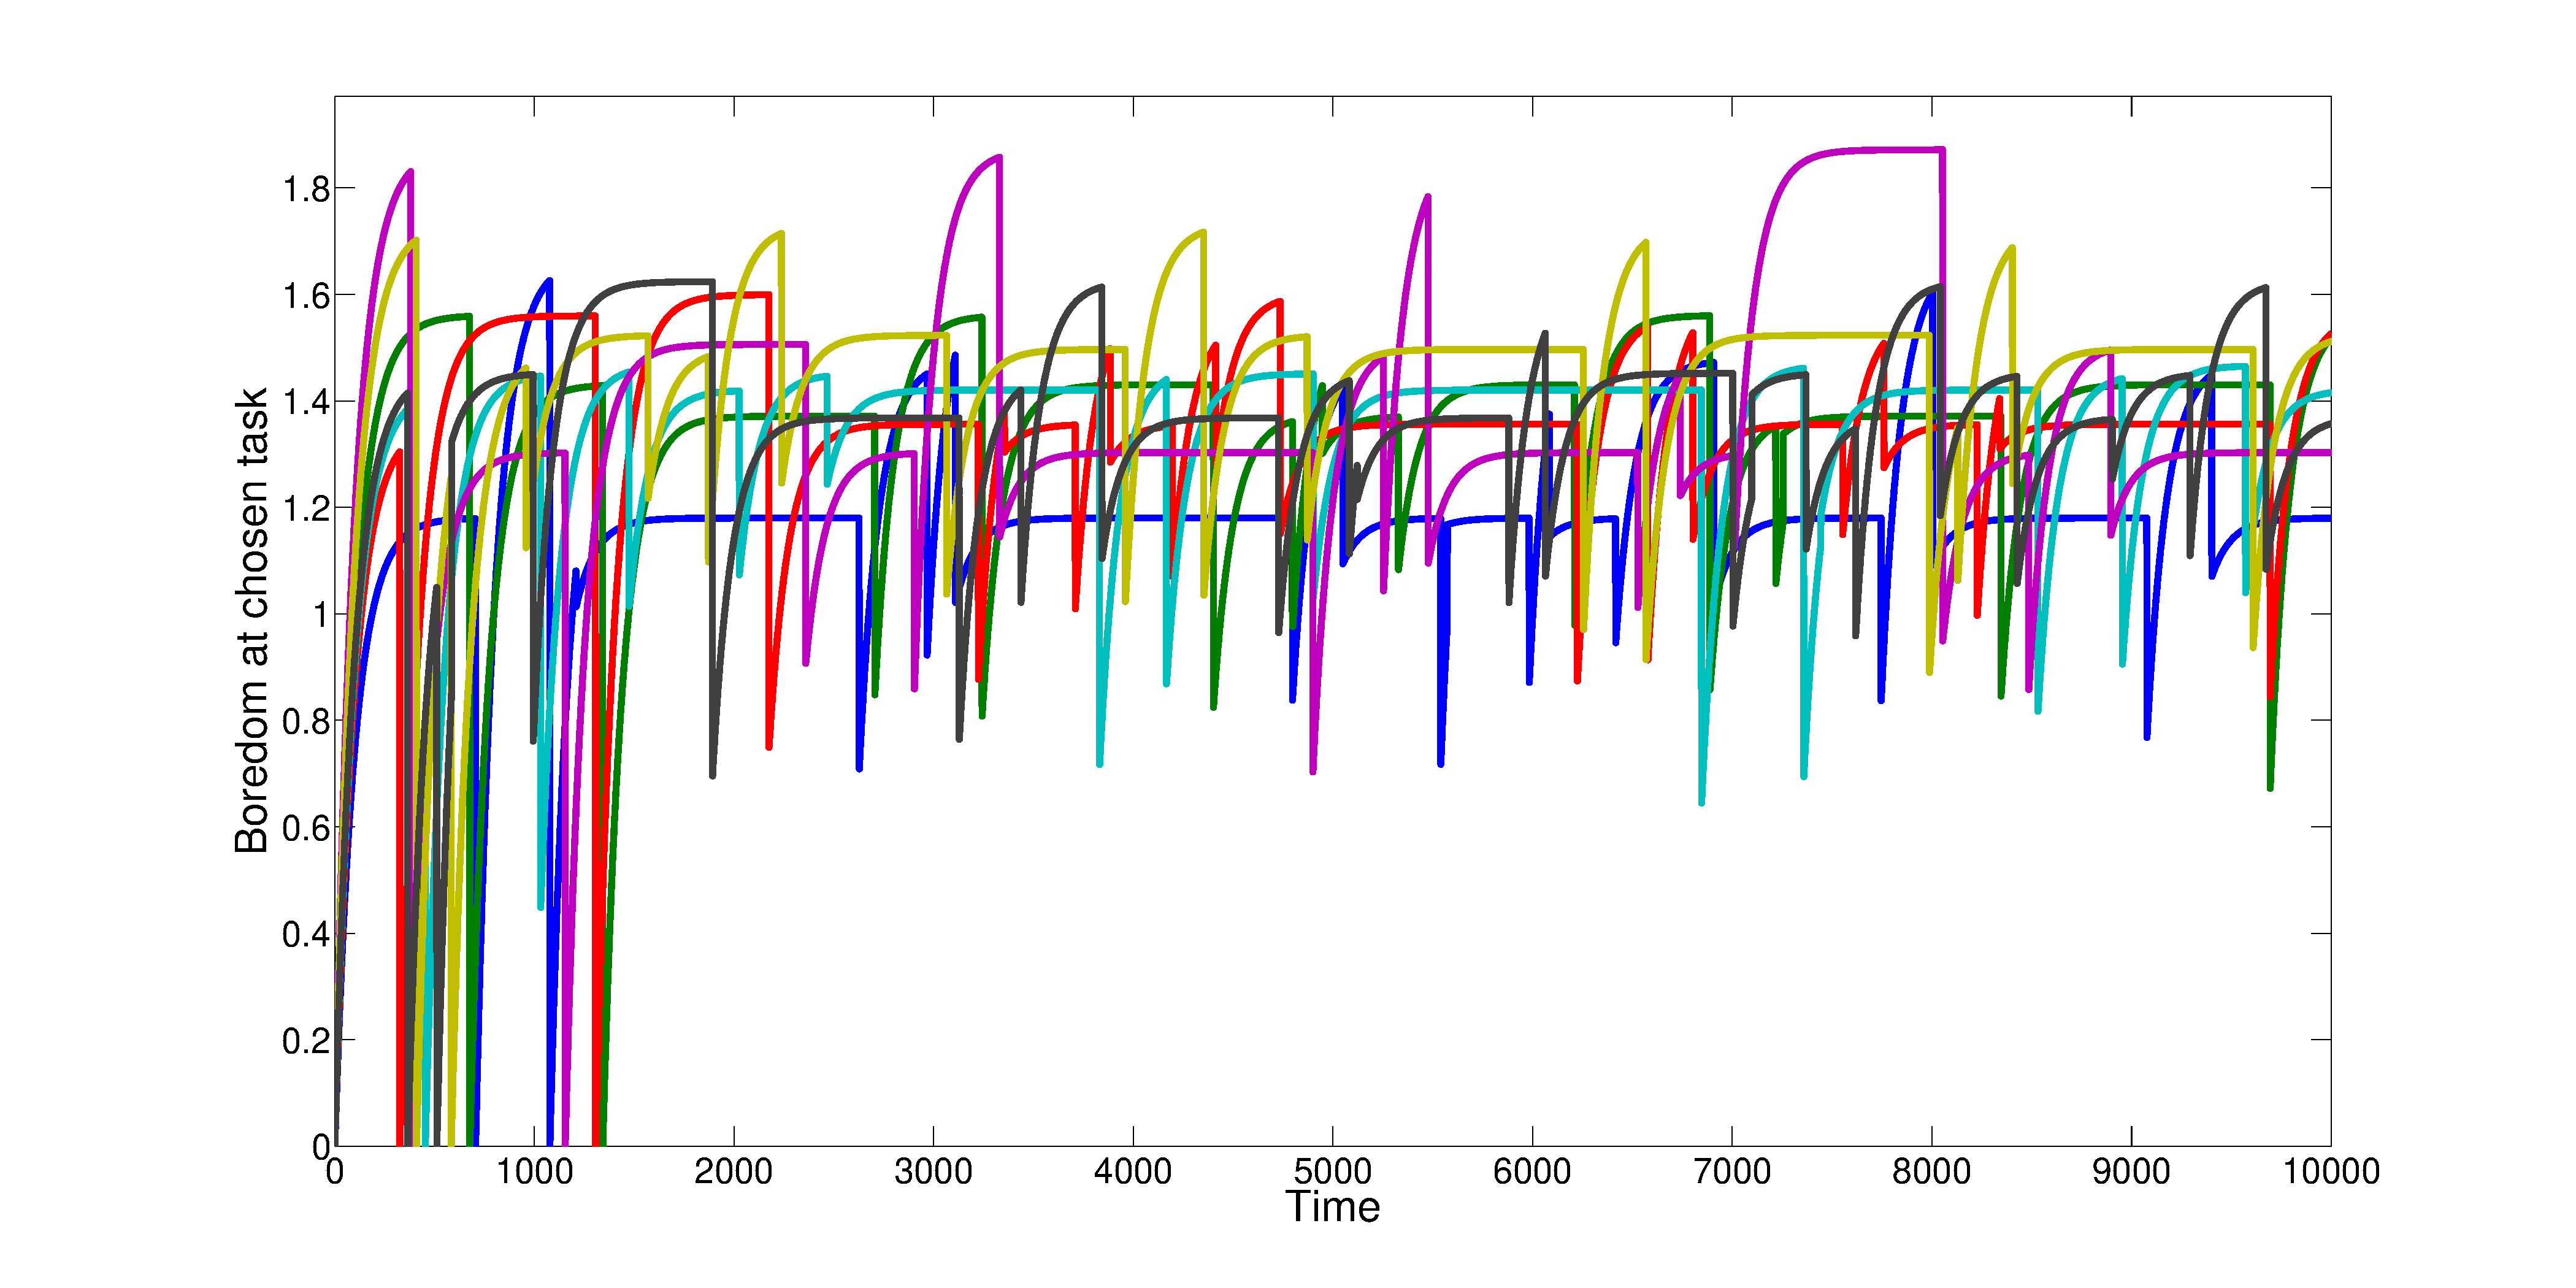
\includegraphics[width=0.9\textwidth]{../figures/moreboredom2.pdf}
	\caption{Boredom experienced by the workers at their current task for high maximal boredoms and a high fatigability.}
	\label{fig:moreboredom2}
\end{figure}

\begin{figure}[hp!]
	\centering
	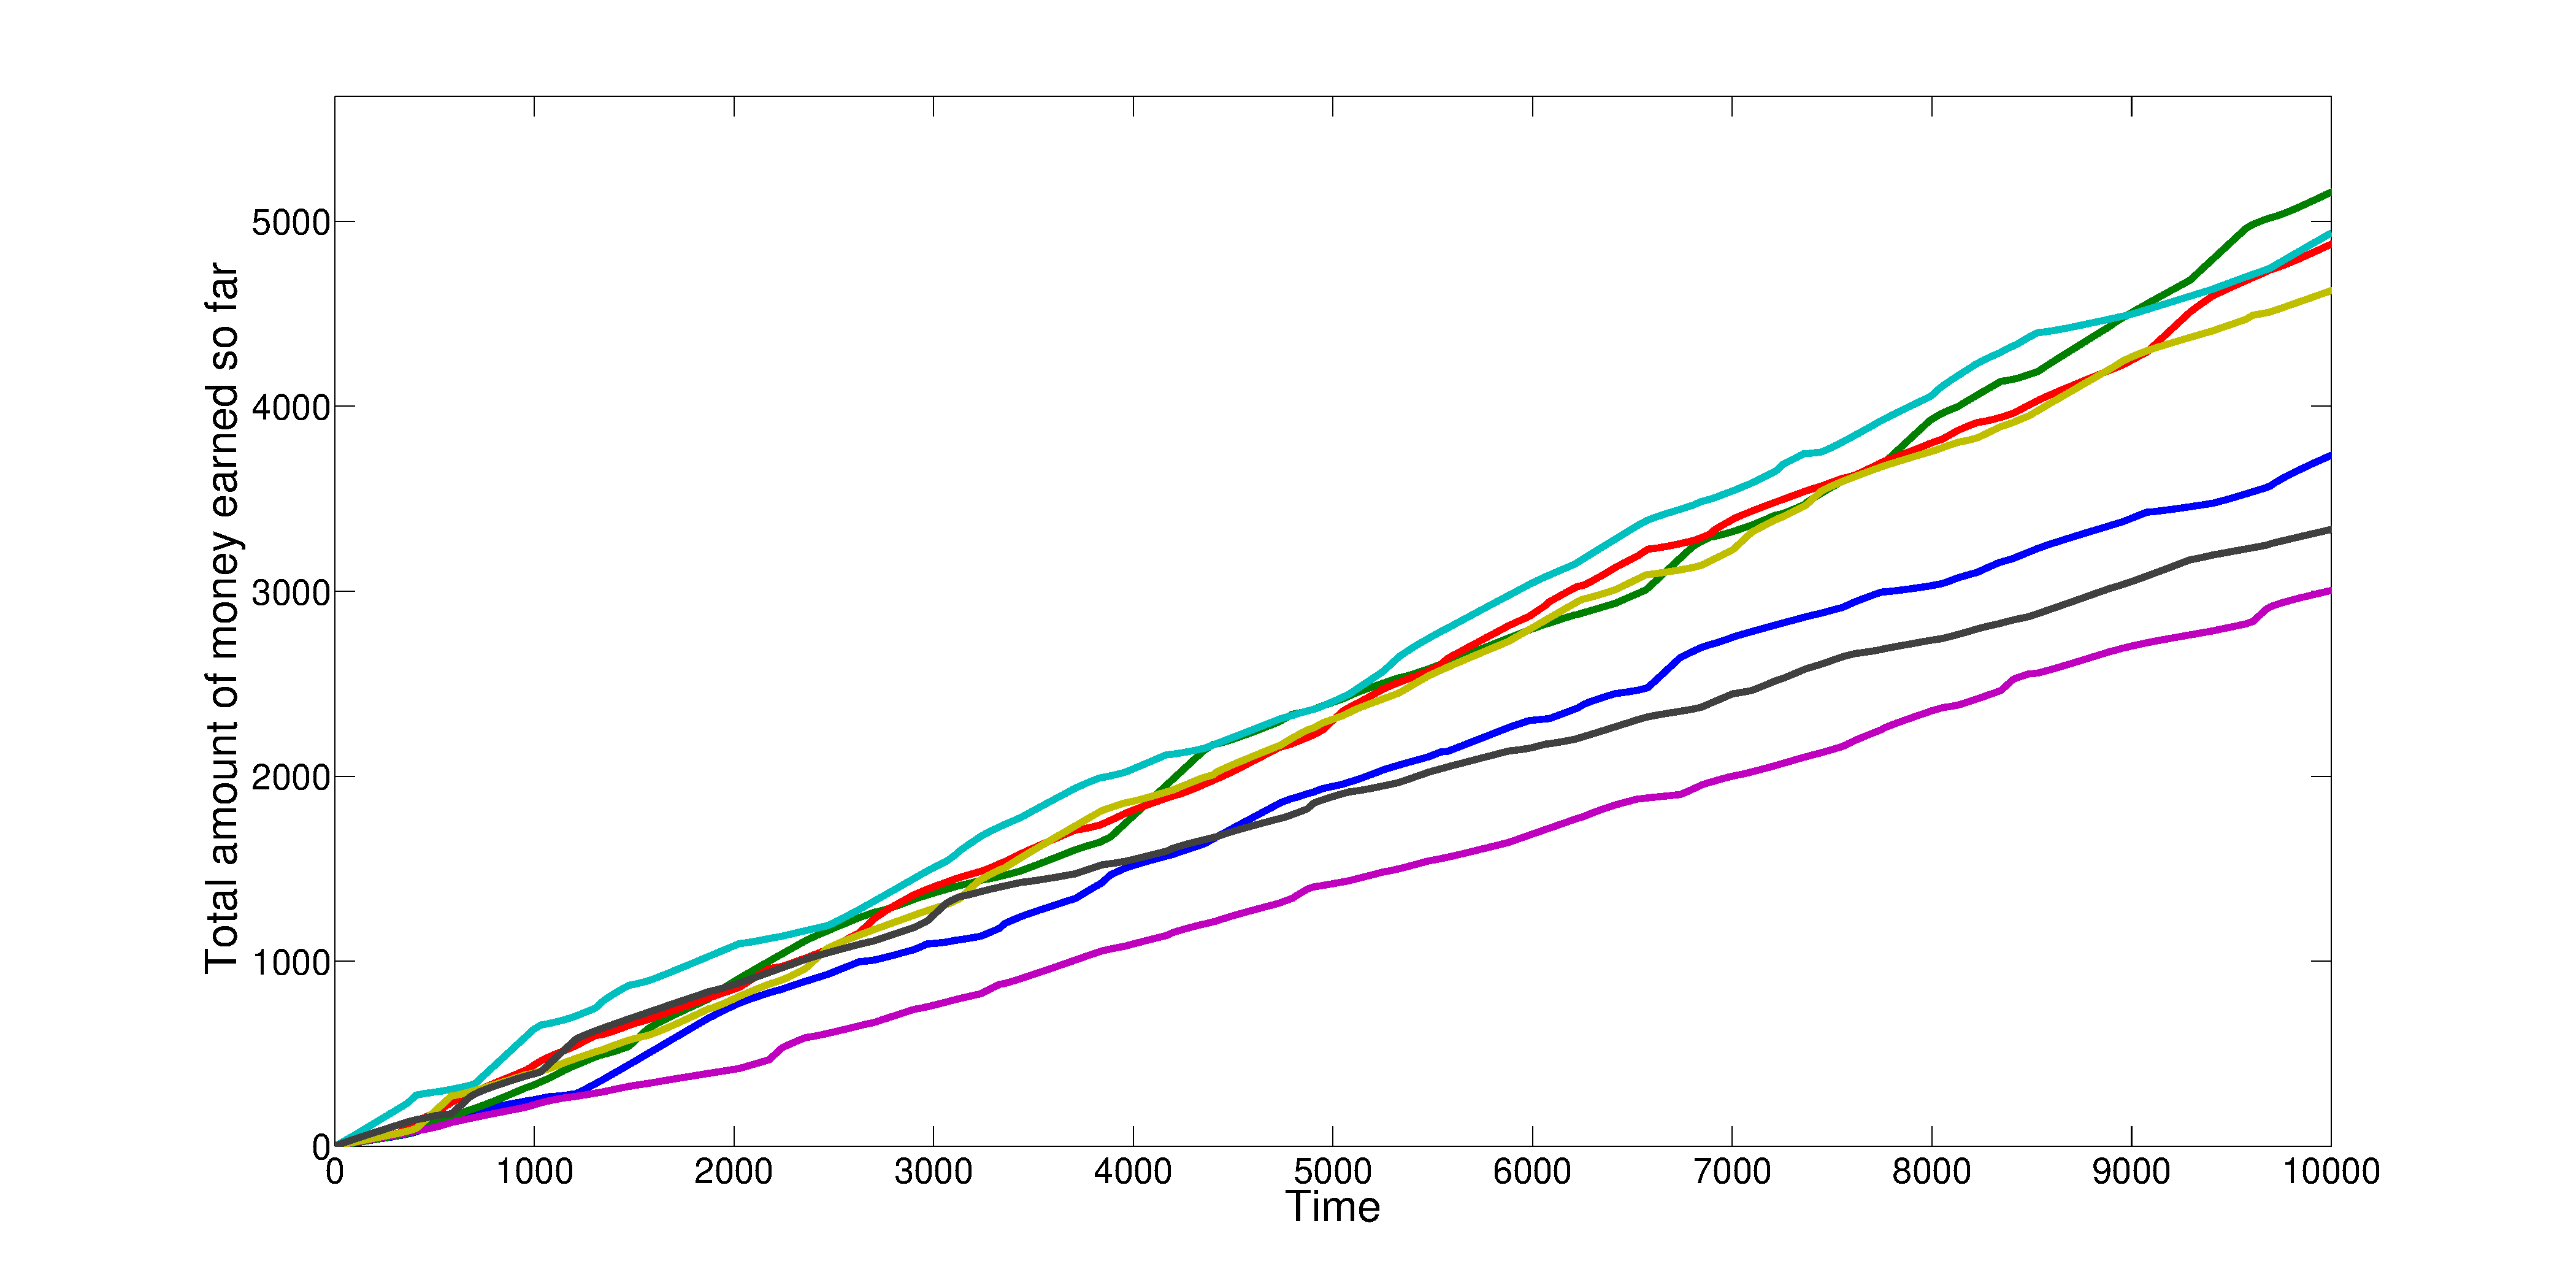
\includegraphics[width=0.9\textwidth]{../figures/moreboredom3.pdf}
	\caption{Total amount of money earned by the workers in the case where the fatigability and the maximal boredoms are high. Despite more fluctuations in comparison with Figure~\ref{fig:sim1totalmoney}, the social inequalities are still pronounced.}
	\label{fig:moreboredom3}
\end{figure}

The parameter $p_s$ becomes important when task changes become frequent and a smaller value for $p_s$ will result in less frequent task changes. However, changing $p_s$ above a specific threshold will have a negligible influence, as the additional time a worker has to wait after a new task has become more profitable will change only little.
